% ---------------------------------------------------------------
% ---------------------------------------------------------------
% This template was developed for the working paper series of 
% the Interdisciplinary Laboratory of Computational Social Science (iLCSS)
% at the University of Maryland, College Park

% The template was built based on  the PNAS Latex model. 

% Adjustments were made by Tiago Ventura, Ph.D. Student in Political Science at UMD, 
% and researcher at the iLCSS.

\documentclass[9pt,twocolumn,twoside]{ilcss}
\usepackage{comment}
\usepackage{graphicx}
\usepackage{amssymb}
\usepackage{epigraph}
\usepackage{amsmath}
\newcommand\scalemath[2]{\scalebox{#1}{\mbox{\ensuremath{\displaystyle #2}}}}

\DeclareMathOperator*{\argmax}{argmax}

\graphicspath{ {./images/} }


\templatetype{ilcssworkingpaper} % Choose template 

\title{Bitcoin Econometrics}	

% Use letters for affiliations, numbers to show equal authorship (if applicable) and to indicate the corresponding author
\author[a]{Gavin Trebilcock}
\author[b]{Tianjiao Li} 
\author[c]{Minghan Shi}

\affil[a]{gt322, Computer Science}
\affil[b]{tl787, Mechanical Engineering}
\affil[c]{ms3536, Electrical and Computer Engineering}

% Please give the surname of the lead author for the running footer
\leadauthor{Gavin} 

% Please include corresponding author, author contribution and author declaration information
\begin{comment}
\authorcontributions{Please provide details of author contributions here.}
\authordeclaration{Please declare any conflict of interest here.}
\end{comment}

\begin{comment}
\equalauthors{\textsuperscript{1}The authors contributed equally to this work.}
\end{comment}

\begin{comment}
\correspondingauthor{\textsuperscript{2}To whom correspondence should be addressed. E-mail: author.two\@email.com}
\end{comment}

\begin{comment}
% Keywords are not mandatory, but authors are strongly encouraged to provide them. If provided, please include two to five keywords, separated by the pipe symbol, e.g:
\keywords{Keyword 1 $|$ Keyword 2 $|$ Keyword 3 $|$ ...}
\end{comment}

\begin{abstract}
In the world of cryptocurrencies, fortunes tend to move up and down quickly. Among them, bitcoin is the original cryptocurrency and it remains the go-to leader of the market. Nevertheless, it is extremely hard to predict the price of bitcoin through standard economic theories, because on bitcoin markets, absent are several features of currency supply and demand, which usually form the basis of currency price. In this report, we present the current progresses in our study of bitcoin market price under the effects of several potential factors. We first show the data retrieval procedures as well as the data visualization, and then present our preliminary data analysis.
\end{abstract}

% \dates{This manuscript was compiled on \today}

% You can change the link on the footer here

\doi{\url{https://github.com/gtrebilcock/BitcoinEconometrics/}}

\begin{document}

\maketitle
\thispagestyle{firststyle}
\ifthenelse{\boolean{shortarticle}}{\ifthenelse{\boolean{singlecolumn}}{\abscontentformatted}{\abscontent}}{}

% If your first paragraph (i.e. with the \dropcap) contains a list environment (quote, quotation, theorem, definition, enumerate, itemize...), the line after the list may have some extra indentation. If this is the case, add \parshape=0 to the end of the list environment.

\dropcap{C}ryptocurrencies have posed great challenges and opportunities for  policymakers, economists, entrepreneurs and consumers since its introduction by Nakamoto \cite{Dyhrberg2016}. The most prominent among them is bitcoin, both in terms of an impressive price development and market capitalisation. However, the price formation of bitcoin cannot be explained by standard economic theories, such as future cash-flows model, purchasing power parity, or uncovered interest rate parity, because several features of currency supply and demand, which usually form the basis of currency price, are absent on bitcoin markets \cite{Ciaian2016}.

We are interested in researching whether or not we can predict the price movement of bitcoin using other public available data. More specifically we are interested testing whether certain metrics which theoretically should be correlated with bitcoin price have any predictive power to determine the prediction of bitcoin prices in the future. 

To do this, we first select candidate factors which potentially have impact on the bitcoin pricing, such as 1. U.S equity market, 2. Graphics Processing Unit (GPU) pricing, 3. U.S inflation rate 4. U.S interest rates, 5. Gold prices 6. Volatility Index. Then we retrieve the corresponding data set from the Internet and visualize the data to obtain an intuitive observation of them. Next, we do feature engineering and do exploratory data analysis of the features to obtain an intuition of the statistical properties of the data. Finally, we truncate the data into training data $\mathcal{D}_{train}$ and testing data $\mathcal{D}_{test}$, fit a simple linear model to the data, and analyze the learning results. We close this report with a discussion section, including remarks on the current results and issues, and our future plan of this project.

\section*{Important Statement}
\textbf{The authors are well aware that the prediction of bitcoin has been an prominent area of study yet there has been no super effective model for such prediction. In this sense, the reported prediction method may not, or won't perform as well as expected. However, the purpose of this study mainly lies in practicing and utilizing the basics of learning theories in a real-world problem. In the meantime, the authors anticipate understanding the underlying difficulties of predicting the bitcoin price from a practical perspective.}

\section{Selection of Explanatory Variables}
We use the overall U.S equity market as a predictor for future bitcoin prices as the U.S equity market generalizes the overall health of the economy, consumer confidence and other socio-political factors that will influence bitcoin pricing. We selected the S\&P as the approximation for the overall U.S equity market as it is a market capitalization weighted fund, which is believed to give a good approximation for the overall health of the market rather than older indexes such as the Dow Jones Industrial Average which is price weighted.  

GPU pricing is another indicator for the prediction of bitcoin pricing in our hypothesis as GPU’s are the primary input cost in mining bitcoins. It is prohibitively difficult to find a data set that tracks GPU component pricing, as there are many different models from different companies available. Instead, we elect to approximate this factor using the stock price of the world’s largest producer of GPU’s, Nvidia.

We also consider the U.S inflation rate as a candidate for the indicator. One of the most valuable characteristics of bitcoin is the finite supply which cannot be manipulated by governmental entities. Therefore we expect to find a correlation between inflation rates and bitcoin prices as some investors use finite supply assets to hedge risk from inflation.

Interest rates are also considered as a potential factor influencing the bitcoin pricing, as currencies are priced against one another based on the interest rate in that country and the financial standing of that country. Accordingly, since we are measuring bitcoin per U.S dollar, it is reasonable to add the variable of U.S interest rates into our model. We chose the 3-month LIBOR as our metric to track daily interest rate changes.

We expect to the spot price of gold to be an important indicator in predicting bitcoin prices. The selection of this asset has many dimensions which are equivalent to bitcoin, including most notably its finite supply. As of October 2019, roughly 18 million bitcoins have been mined of the 21 million total available as reported by \url{blockchain.com/charts/total-bitcoins?timespan=all}. Historically, gold was used as a currency and is still being used as a store of wealth. Bitcoin shares similar characteristics as it is currently being used as a store of wealth and is attempting to make its way into the arena of currencies on a global level.

Finally, we use the volatility index as an approximation of the fear indicator in the market. As we have stated previously, bitcoin is treated by many investors as a safe haven for assets in times of market volatility. The volatility index represents the expected range of price volatility in the S\&P 500 index roughly over the next month and a single standard deviation of confidence.  

\section{Retrieval of Data}
We retrieved daily bitcoin pricing (Figure \ref{BTC_GSPC_NVDA_Gold} (a)) from \url{https://coinmarketcap.com/currencies/bitcoin/historical-data/} which is a database that tracks many cryptocurrencies. The site offers the longest history on Bitcoin pricing that we were able to find dating back to April 28, 2013.

Our S\&P500 (Figure \ref{BTC_GSPC_NVDA_Gold} (b)) and Nvidia daily price data (Figure \ref{BTC_GSPC_NVDA_Gold} (c)) were extracted from Yahoo finance and are measured in USD. Yahoo finance offers adjusted close prices which adjust daily close prices for dividends and stock splits. This makes the calculation for daily returns much simpler. We note that daily data for these two assets are tracked on trading days, which specifically exclude weekends and holidays. This forced us to use approximately 253 data points per year rather than the expected 365. We pulled data only for the dates that aligned with these two assets, as there would be less sparse data to deal with. 

Our daily spot gold pricing (Figure \ref{BTC_GSPC_NVDA_Gold} (d)) was taken from \url{https://perthmint.com/} which provides daily spot pricing for gold priced in United States dollars (USD) per ounce. 

\begin{figure*}
\centering
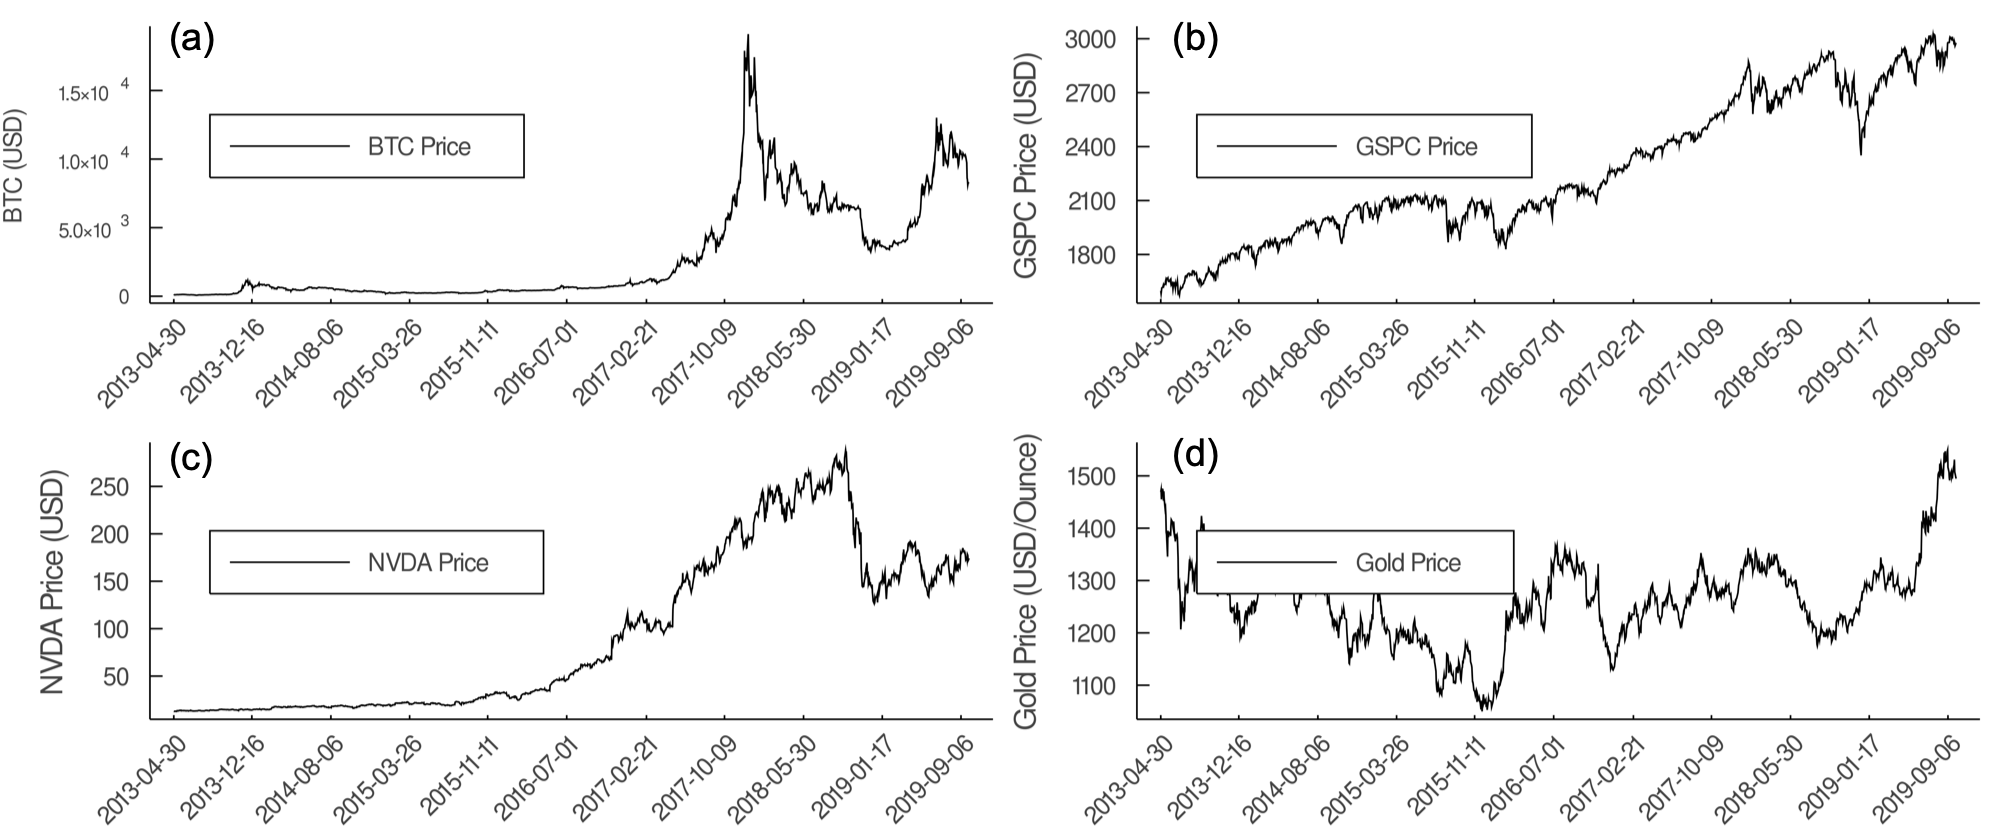
\includegraphics[width=0.85\linewidth]{fig1to4.png}
\caption{(a)The Bitcoin price since April 28, 2013, on a daily basis (retrieved from \url{https://coinmarketcap.com/currencies/bitcoin/historical-data/}) (b)S\&P500 daily price since April 28, 2013, on a daily basis (retrieved from Yahoo finance) (c)Nvidia daily price since April 28, 2013, on a daily basis (retrieved from Yahoo finance) (d)Daily spot gold pricing taken from \url{https://perthmint.com/}.}
\label{BTC_GSPC_NVDA_Gold}
\end{figure*}

We found daily inflation rates from the Federal Reserve Economic Data (FRED) database \url{https://fred.stlouisfed.org/}. This variable is measured daily and the units on each data point is in percentage terms. We also retrieved daily 3-month LIBOR rates from the FRED database. This variable is measured daily and the units on each data point is in percentage terms. 

\begin{figure}[tbhp]
\centering
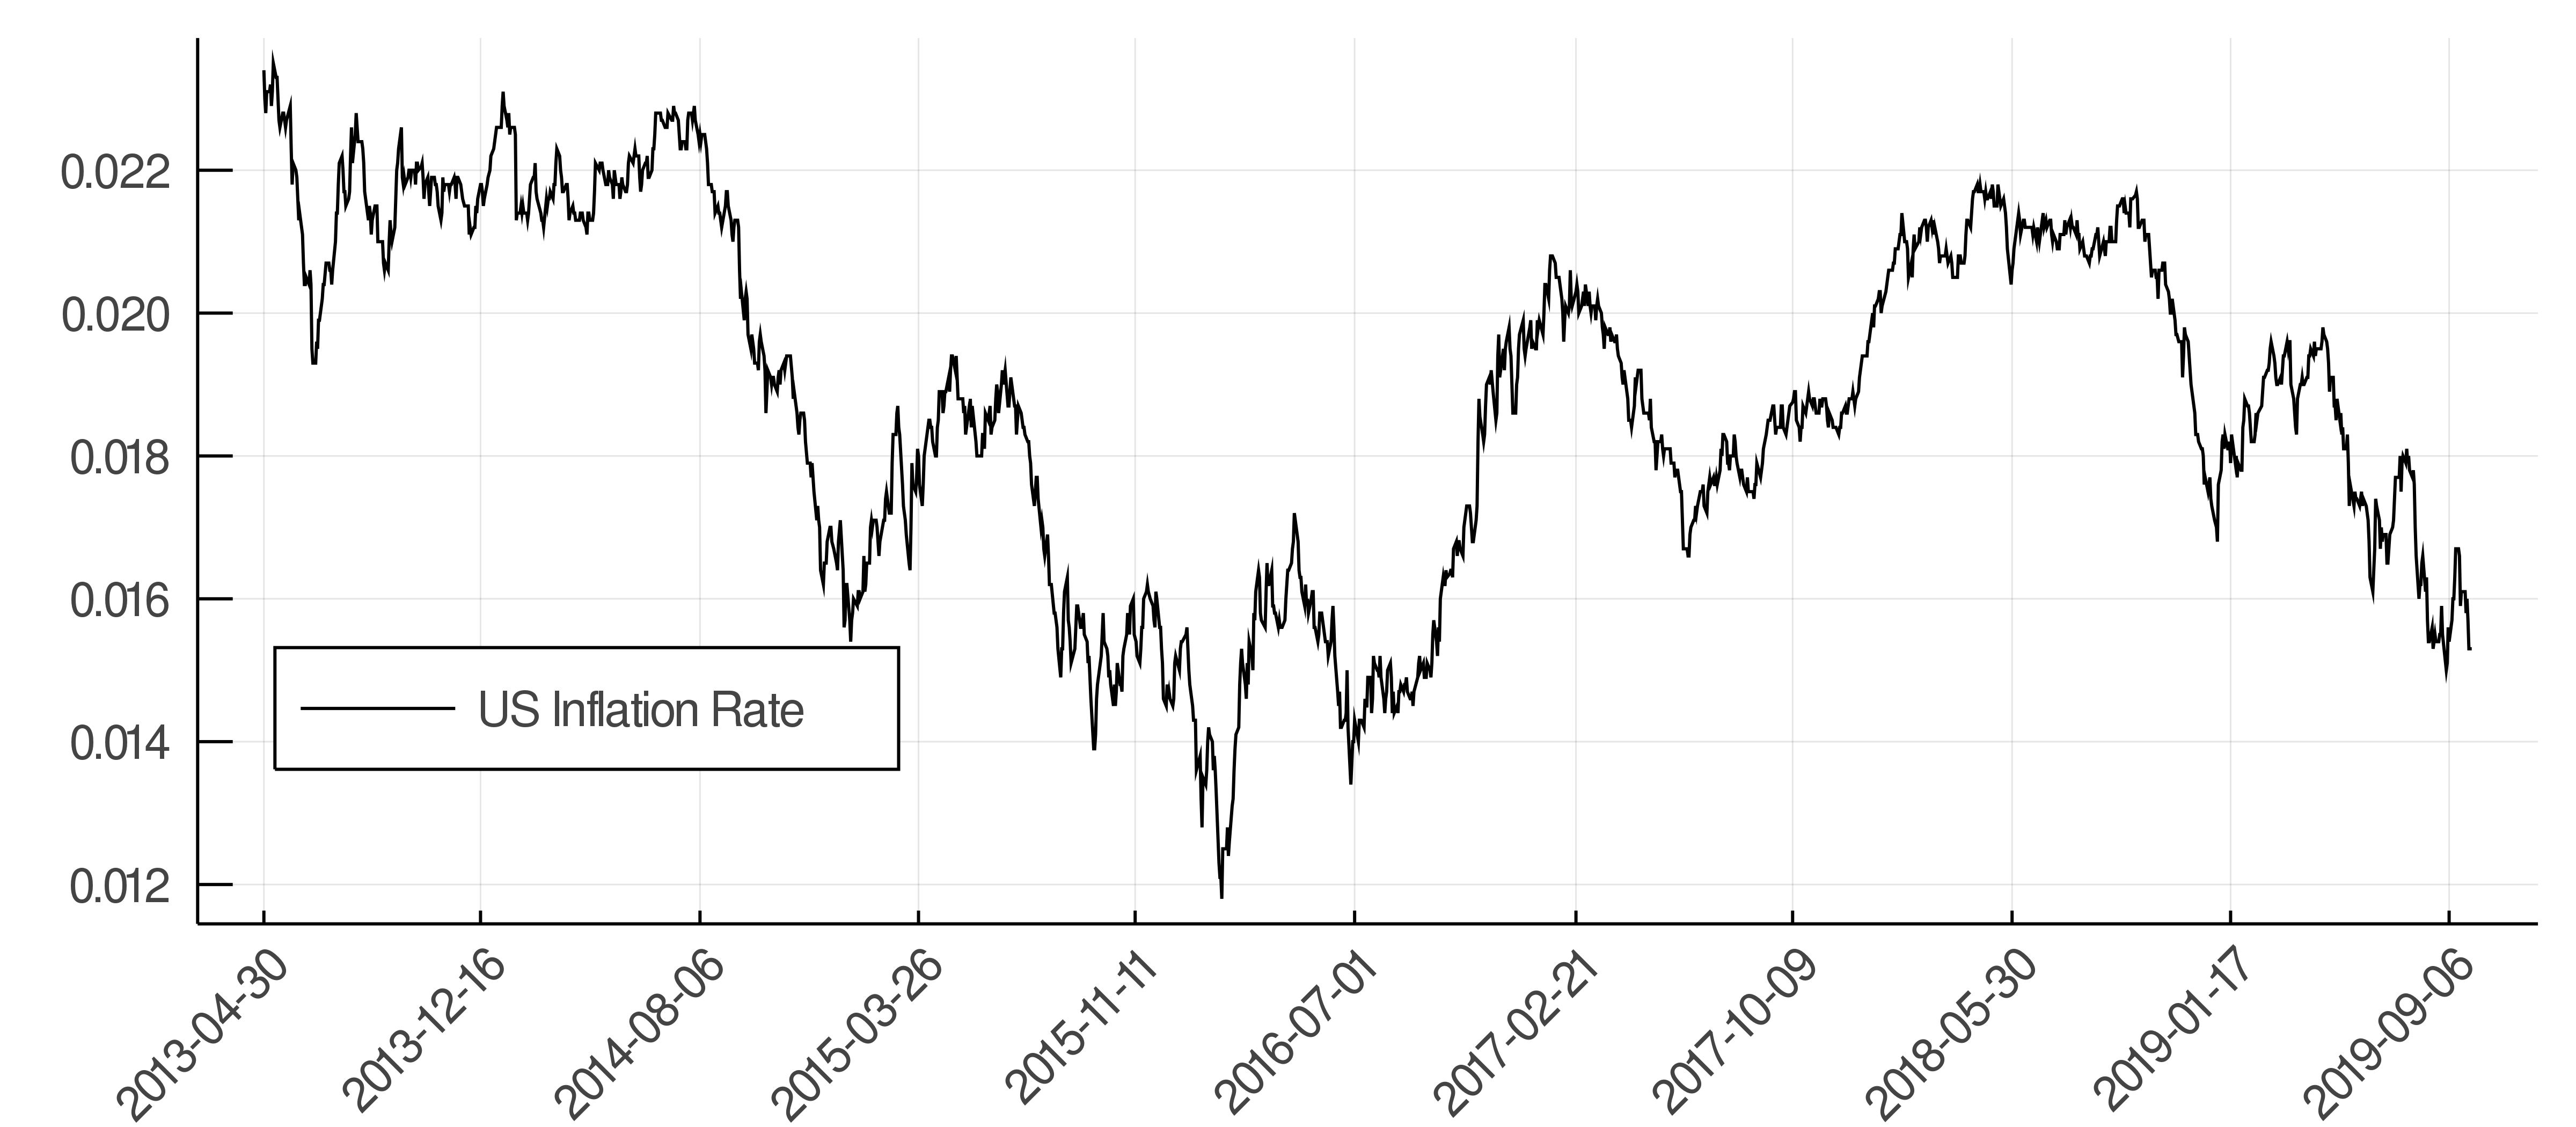
\includegraphics[width=.85\linewidth]{US_inflation_rate.png}
\caption{daily inflation rates from the Federal Reserve Economic Data (FRED) database \url{https://fred.stlouisfed.org/}}
\label{infl_rate}
\end{figure}

\begin{figure}[tbhp]
\centering
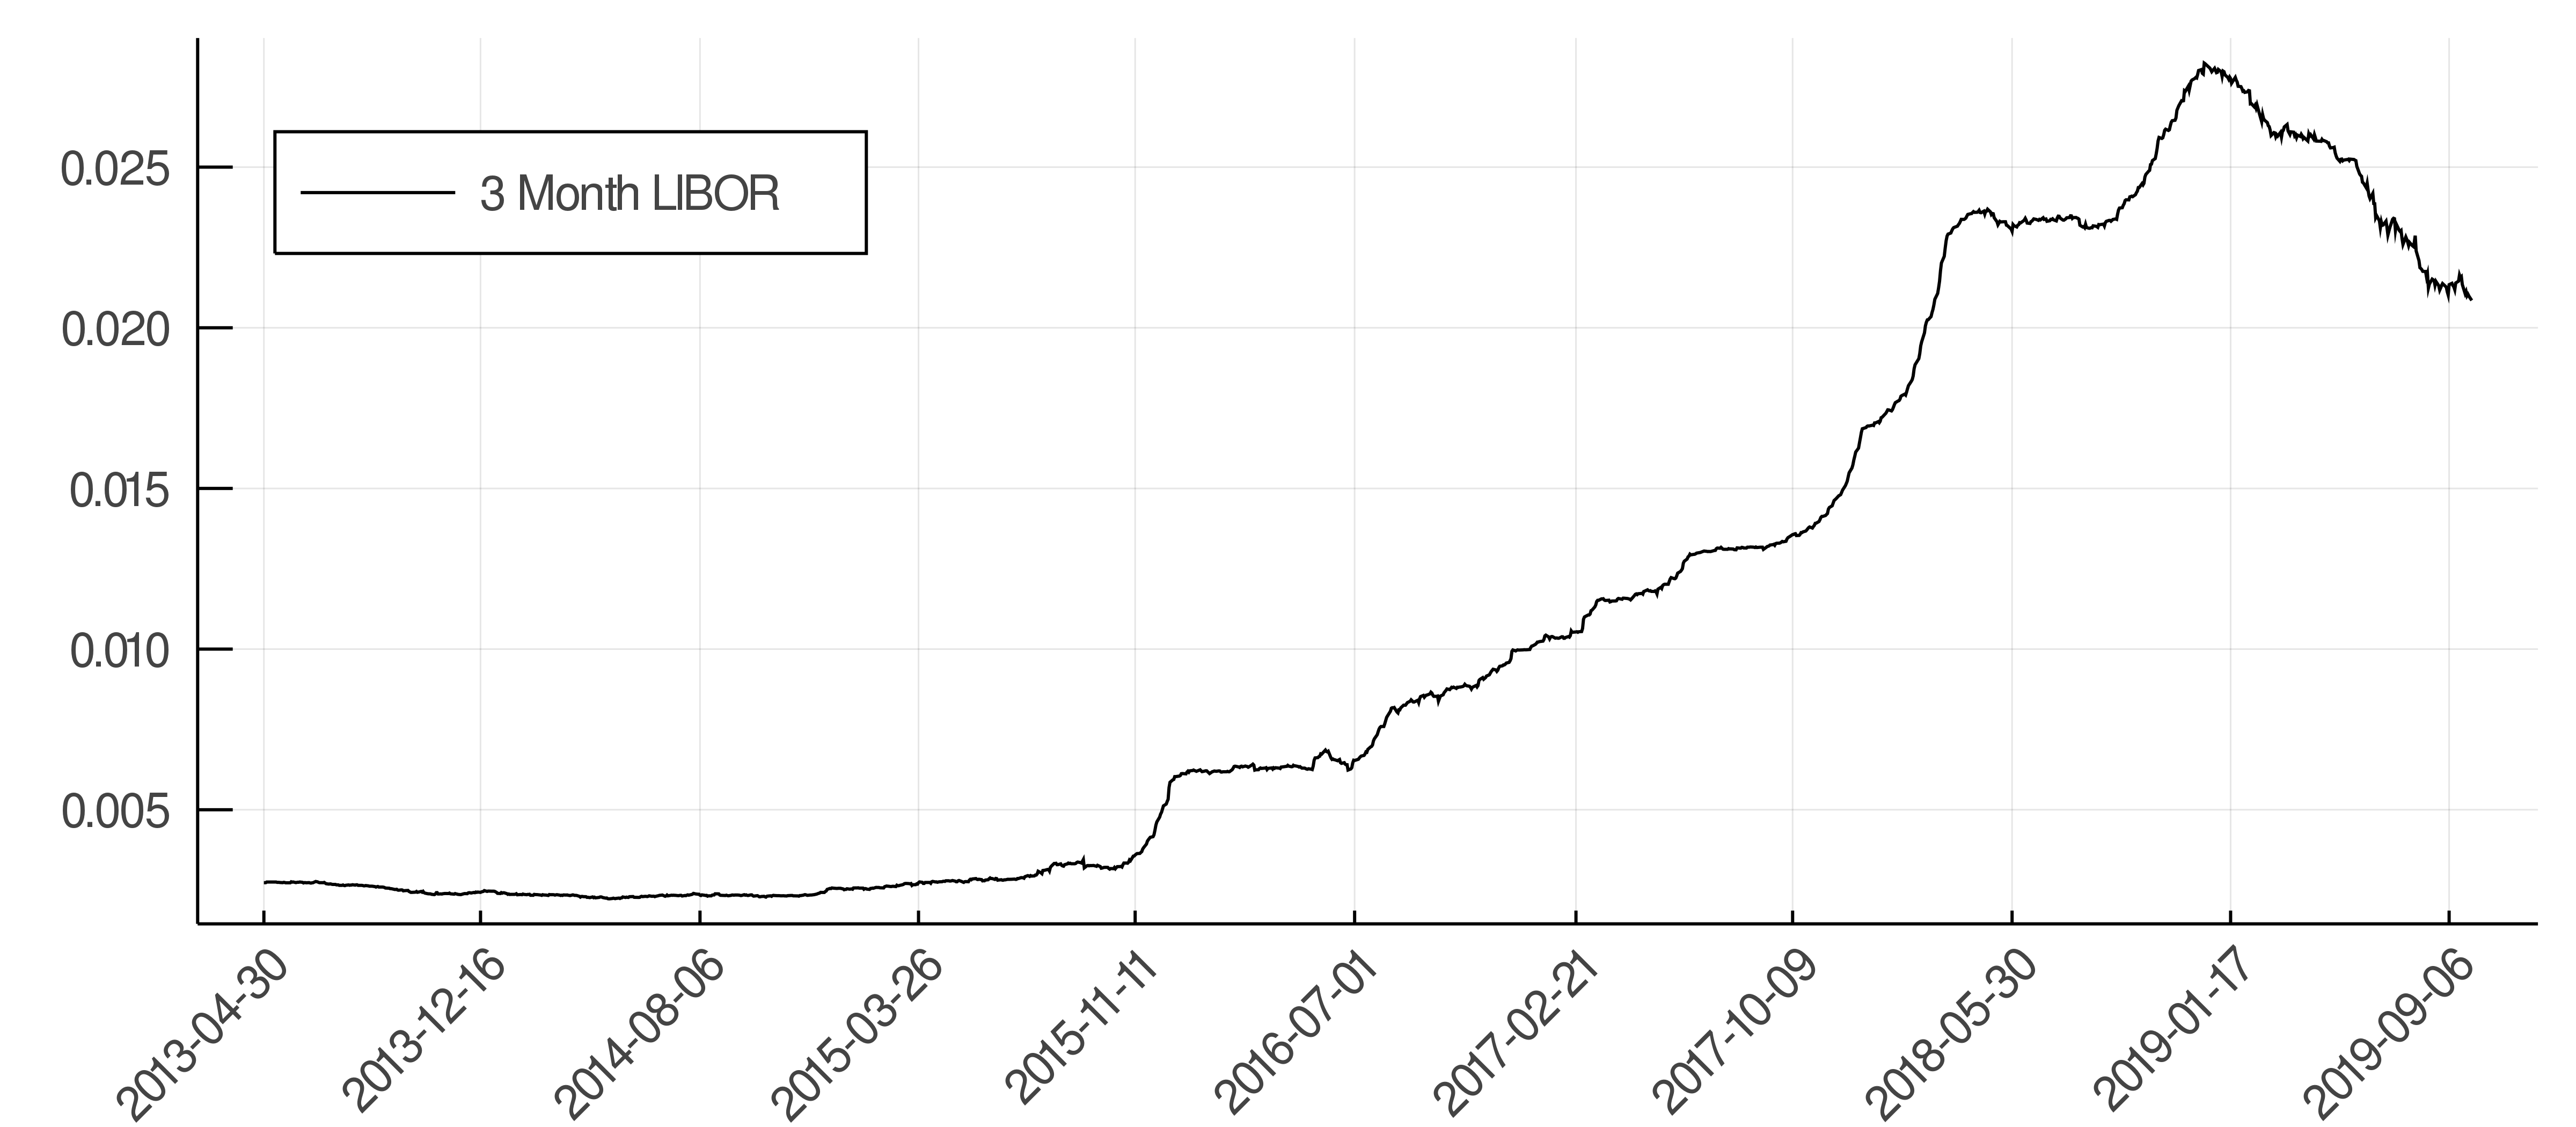
\includegraphics[width=.85\linewidth]{3_month_LIBOR.png}
\caption{Daily 3-month LIBOR rates from the FRED database \url{https://fred.stlouisfed.org/}.}
\label{3m_LIBOR}
\end{figure}

We retrieved daily volatility index (VIX) pricing from the CBOE. This variable is measured daily and the units on each data point is in percentage points.  

\section{Data Summary and Feature Engineering}
\subsection*{Data Summary}
We only considered dates at which we had data for each of these inputs and this was delimited by the number of trading days per year (253). Throughout our data collection process the most common issue we faced was missing data points. This was apparent after we initially plotted the U.S inflation rates over time and there were sudden drops from 1.5\% to 0.0\% in one day, which happened in 11 data points out of 1617 (0.6\%) in this specific data series. We resolved this issue by linearly interpolating the missing data point, calculating the median of the day prior and the day after the missing data point. We also ran into the same issue after we initially plotted spot gold price over time. In this data series we had 24 data points out of 1617 missing (1.5\%), which we resolved through linear interpolation utilizing the same method as was used for missing inflation rate data. We did not run into data corruption issues.
\subsection*{Feature Engineering}
We have 1617 daily data points for each of our explanatory variables and for bitcoin pricing. Currently we are considering 6 explanatory variables. After transformations we will have a total of 19 explanatory variables to consider.
We have added features for the logarithmic returns of assets for bitcoin, Nvidia, GSPC and gold. We chose to calculate daily returns using a logarithmic basis, calculated by the $\ln{\frac{today's price}{yesterday's price}}$. We chose this metric as it presents returns in an additive way, that is if today's return is .01 and yesterday's return was .01, we in total have a .02 return. This is not this case in calculating returns using $\frac{today's price - yesterday's price}{yesterday's price}$. This will be important for our calculations if we consider returns daily over a long period of time. Another feature transformation we added was an auto-regressive term for each of our variables that is lagged 30 days. 

Thus, at the end, we have 11 variables. Those variables, together with their names in the code are listed in Table \ref{var_names}. In the following discussions, the variable names in code may appear in figures/tables/contexts instead of the natural names.

\begin{table}[h]
\centering
\caption{Variables and Corresponding Names}
\label{var_names}
\begin{tabular}{@{\extracolsep{10pt}}ll} 
\hline
\hline
                       & variable name        \\ 
\hline
Bitcoin adjusted price & BTC\_adj\_price      \\
GSPC adjusted price    & GSPC\_adj\_price     \\
NVDA adjusted price    & NVDA\_adj\_price     \\
Gold adjusted price    & Gold\_adj\_price     \\
Bitcoin log return     & BTC\_log\_ret        \\
GSPC log return        & GSPC\_log\_ret       \\
NVDA log return        & NVDA\_log\_ret       \\
Gold log return        & Gold\_log\_ret       \\
U.S inflation rate     & US\_inflation\_rate  \\
3 month LIBOR          & 3\_month\_LIBOR      \\
Volatility index       & VIX                  \\
\hline
\end{tabular}
\end{table}

\section{Exploratory Data Analysis and The Simple OLS Linear Regression}
After feature engineering, we first show the fluctuation of the data by visualizing the distribution of the daily returns (Figure \ref{hist_distribution}) generated in the previous section. We notice that the bitcoin price has the largest daily fluctuations compared to the feature variables. This indicates the bitcoin price forming is complicated and we do not have enough features to capture the bitcoin pricing at this point.

\begin{figure*}[tbhp]
\centering
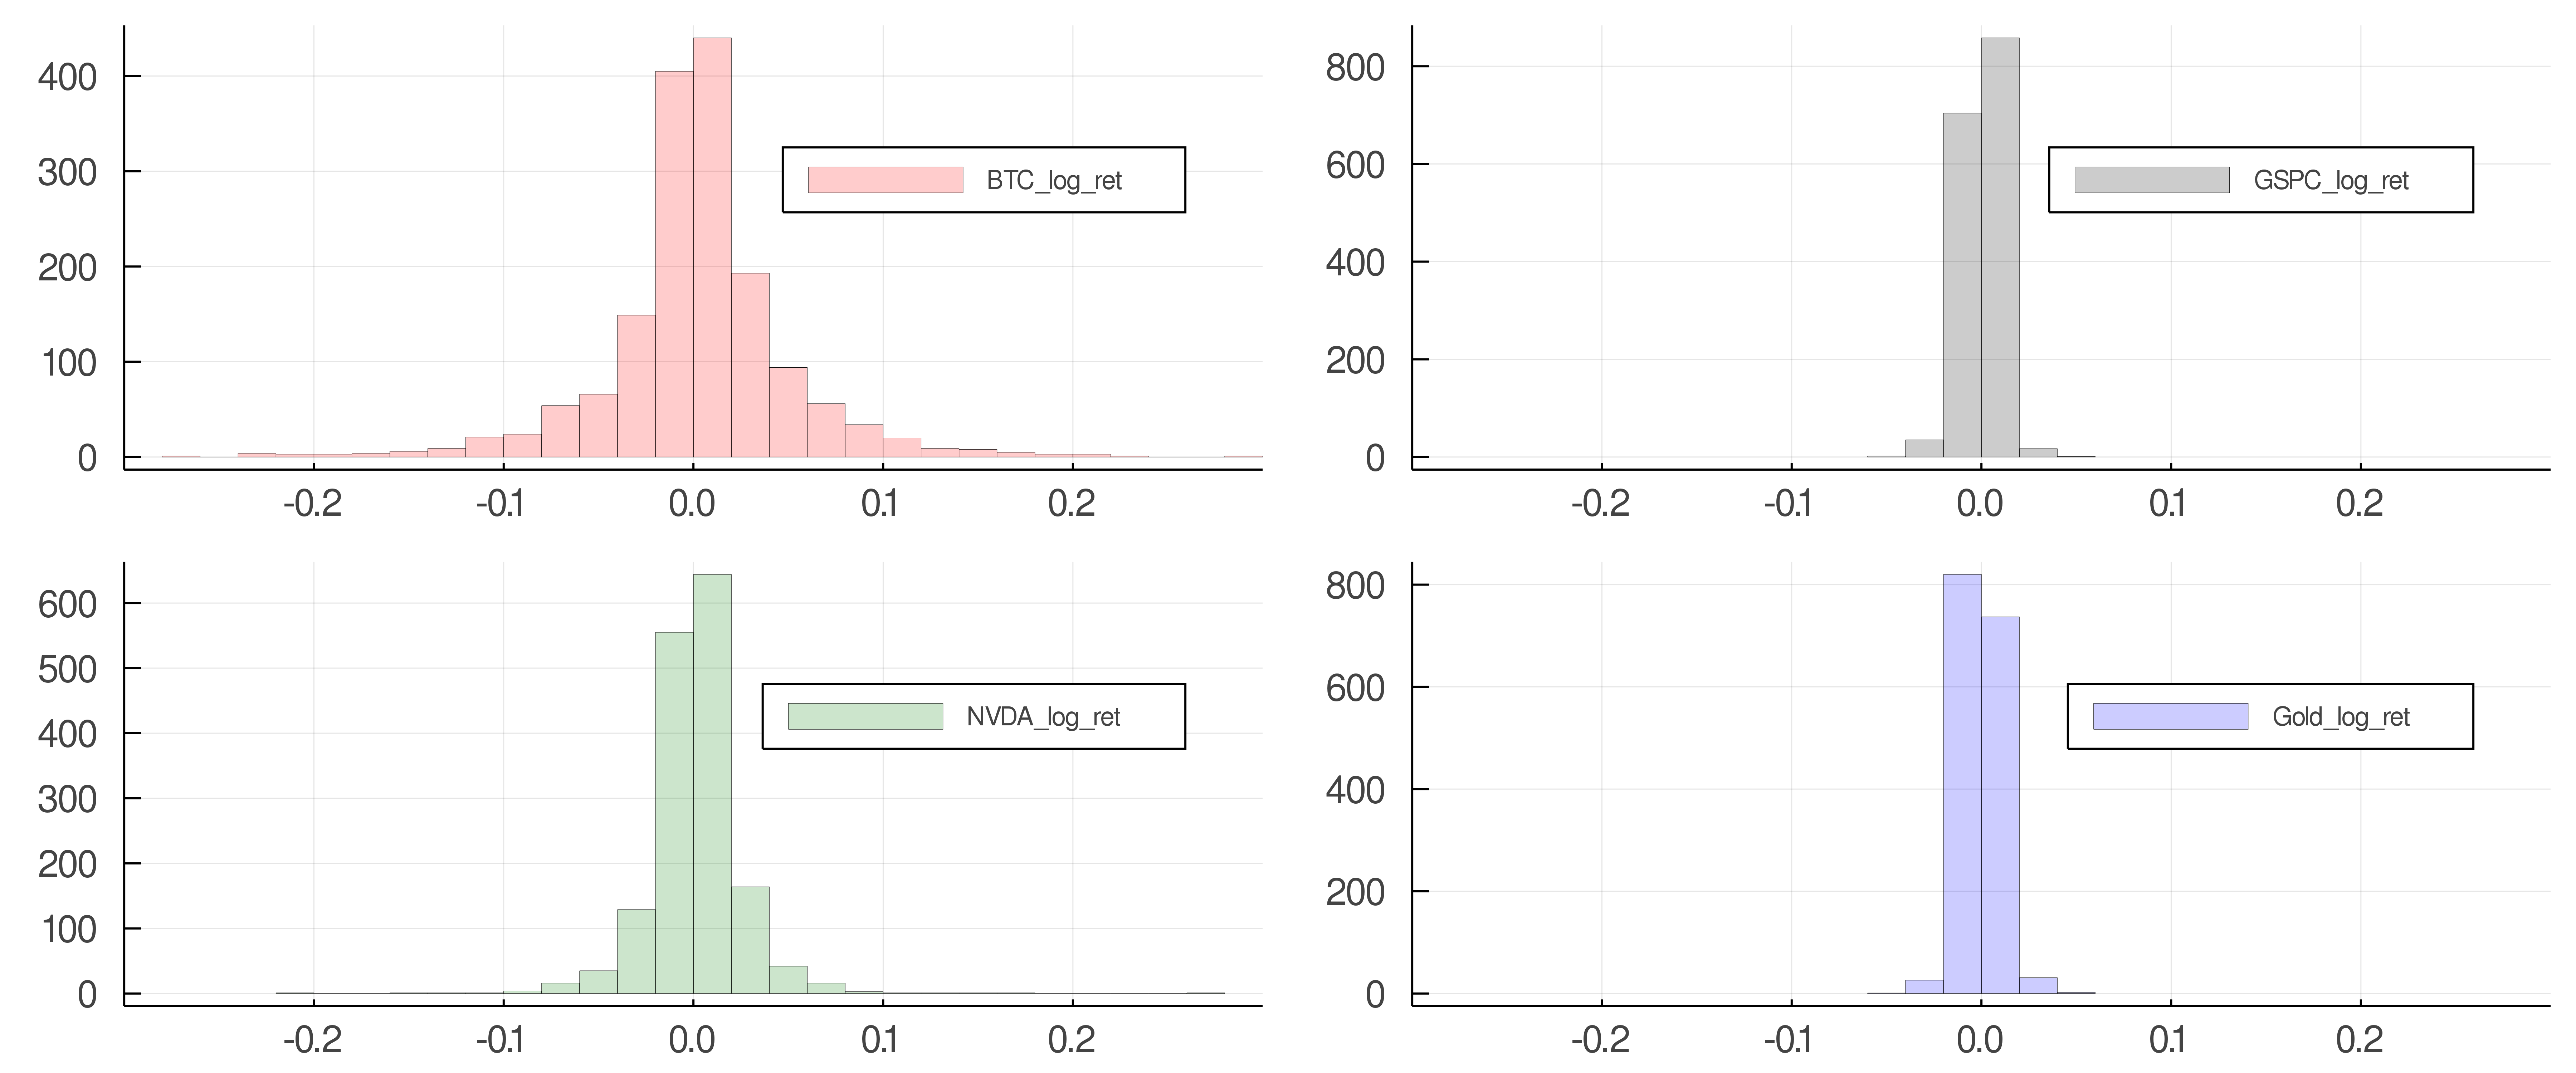
\includegraphics[width=.85\linewidth]{return_hists.png}
\caption{Histograms showing the distributions of the return rate of bitcoin price, GSPC price, NVDA price and gold price.}
\label{hist_distribution}
\end{figure*}

We also do a correlation analysis between the features, shown in Figure \ref{corr}. It is shown that the bitcoin price has relatively strong correlation with the GSPC price, NVDA price, and the 3-month LIBOR. These findings illuminate the feasibility of our study. 

\begin{figure}[h]
\centering
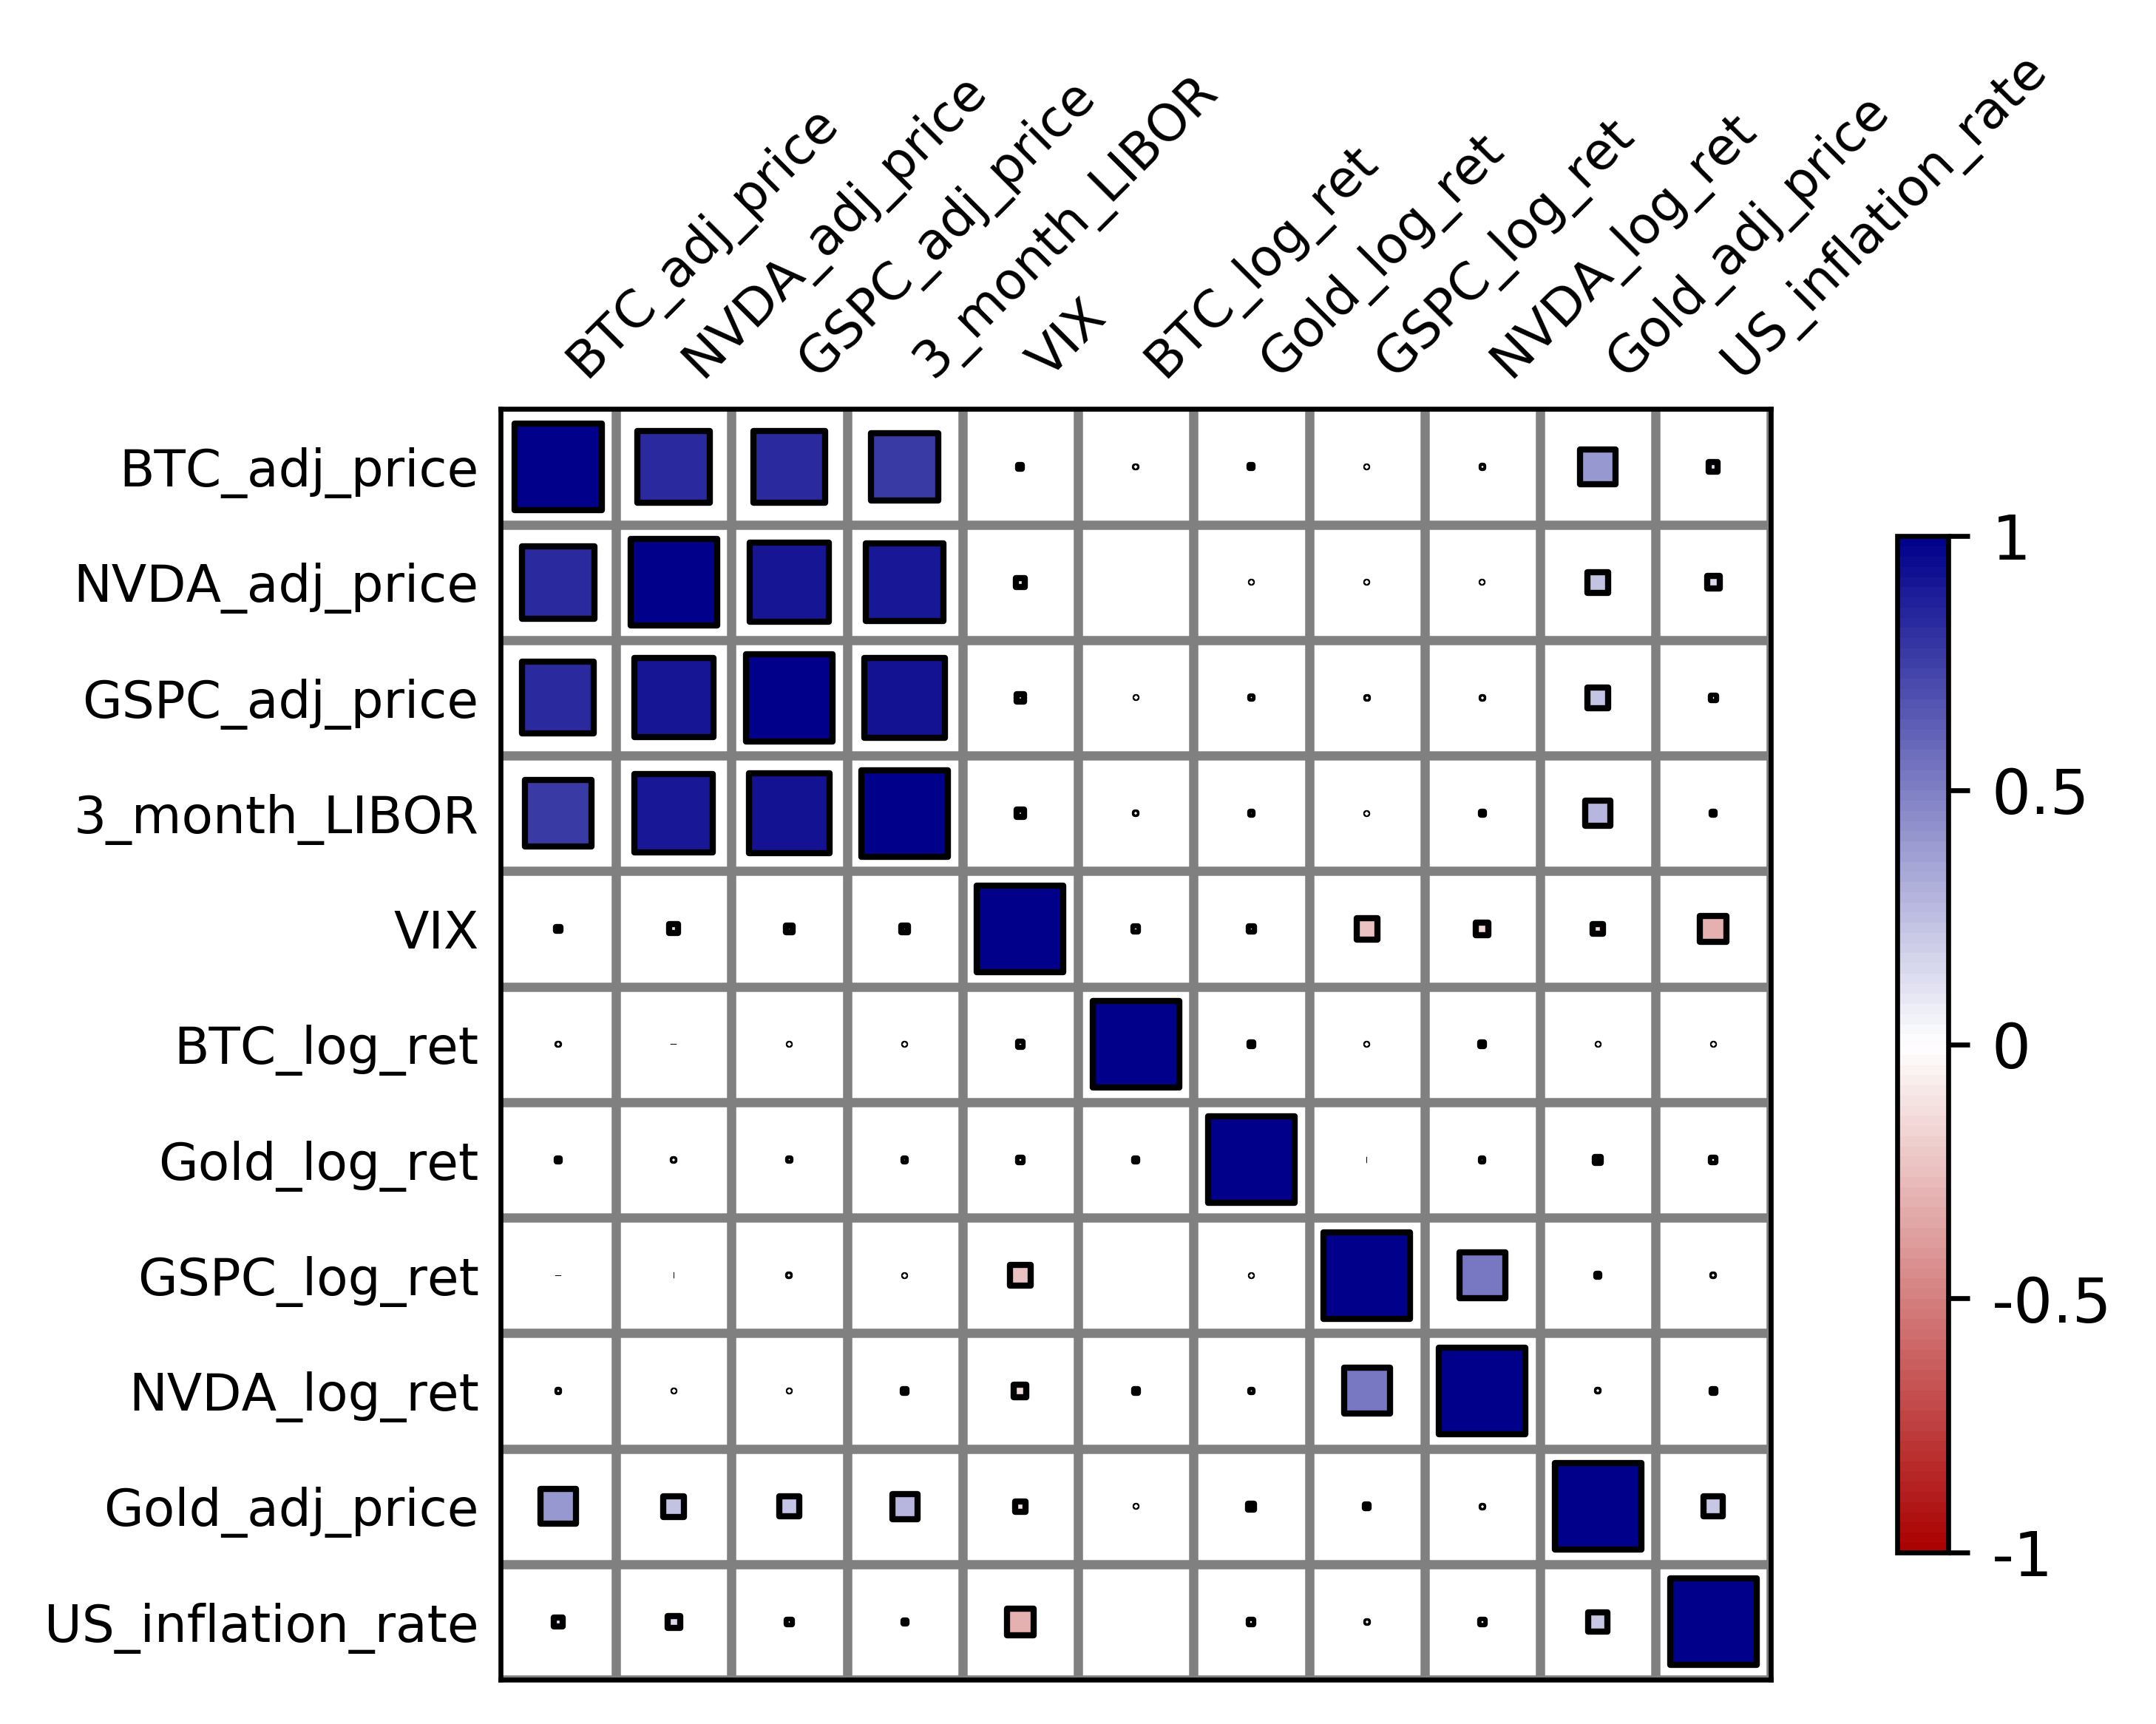
\includegraphics[width=0.8\linewidth]{new_heat_map.png}
\caption{Correlations between the features and the bitcoin price. (via biokit.viz)}
\label{corr}
\end{figure}

The data we have is a time series. Thus, the first 80\% of the data are put into $\mathcal{D}_{train}$ while the most recent 20\% of the data are put into $\mathcal{D}_{test}$. We fit a simple ordinary least squares (OLS) regression with each of our explanatory variables and the results are shown in Figure \ref{reg_no_trans}. It is obvious that this equation has little to no predictive power. We concluded that adding an auto-regressive term based on prior day bitcoin price as today's bitcoin price would be logically sound as tomorrow's bitcoin price will be dependent on today's price. The results from this OLS linear regression are shown in Figure \ref{reg_yes_trans}.

\begin{figure}[h]
\centering
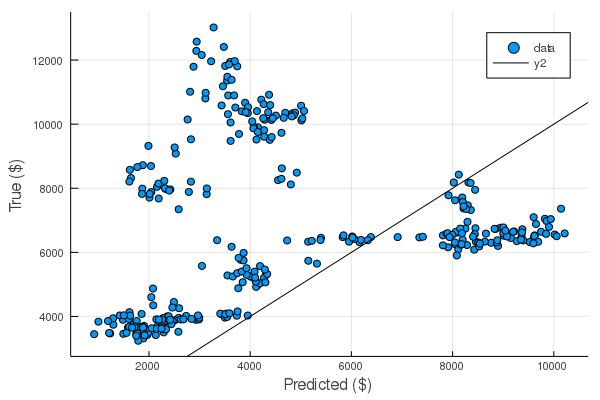
\includegraphics[width=.75\linewidth]{Regression_w_o_lag.png}
\caption{Simple regression without feature transformations. Train MSE: $2.77406e+06$, Test MSE: $1.51665e+07$}
\label{reg_no_trans}
\end{figure}

\begin{figure}[h]
\centering
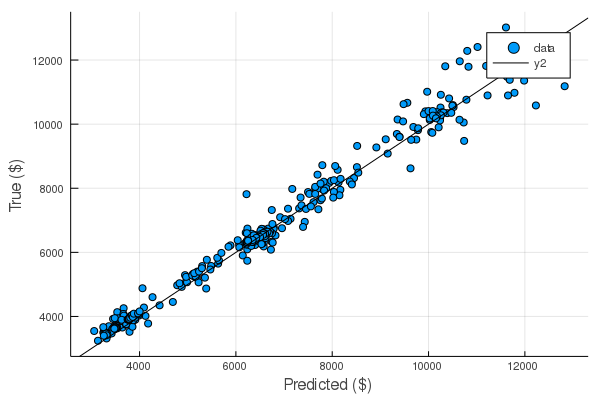
\includegraphics[width=.8\linewidth]{Regression_on_price.png}
\caption{Regression using an autoregressive term of bitcoin price. Train MSE: $70,466.77354$, Test MSE: $148,161.7512$}
\label{reg_yes_trans}
\end{figure}

The simple linear regression fits a prediction line where approximately 50 percent of the data is above the line and the other 50 percent is below the line by definition of ordinary least squares. This means our prediction will be as good as a coin flip for points above the line as well as below the line.
In order to adjust our confidence in predicting positive returns, we fit a quantile regression to our data. In Figure \ref{quantile_reg_price} we run a quantile regression at the fifth quantile. On average, this prediction will under-estimate future prices as 95\% of data will be above our prediction line. We find this classification useful as it could alert investors when asymmetric opportunities appear. 

\begin{figure}[h]
\centering
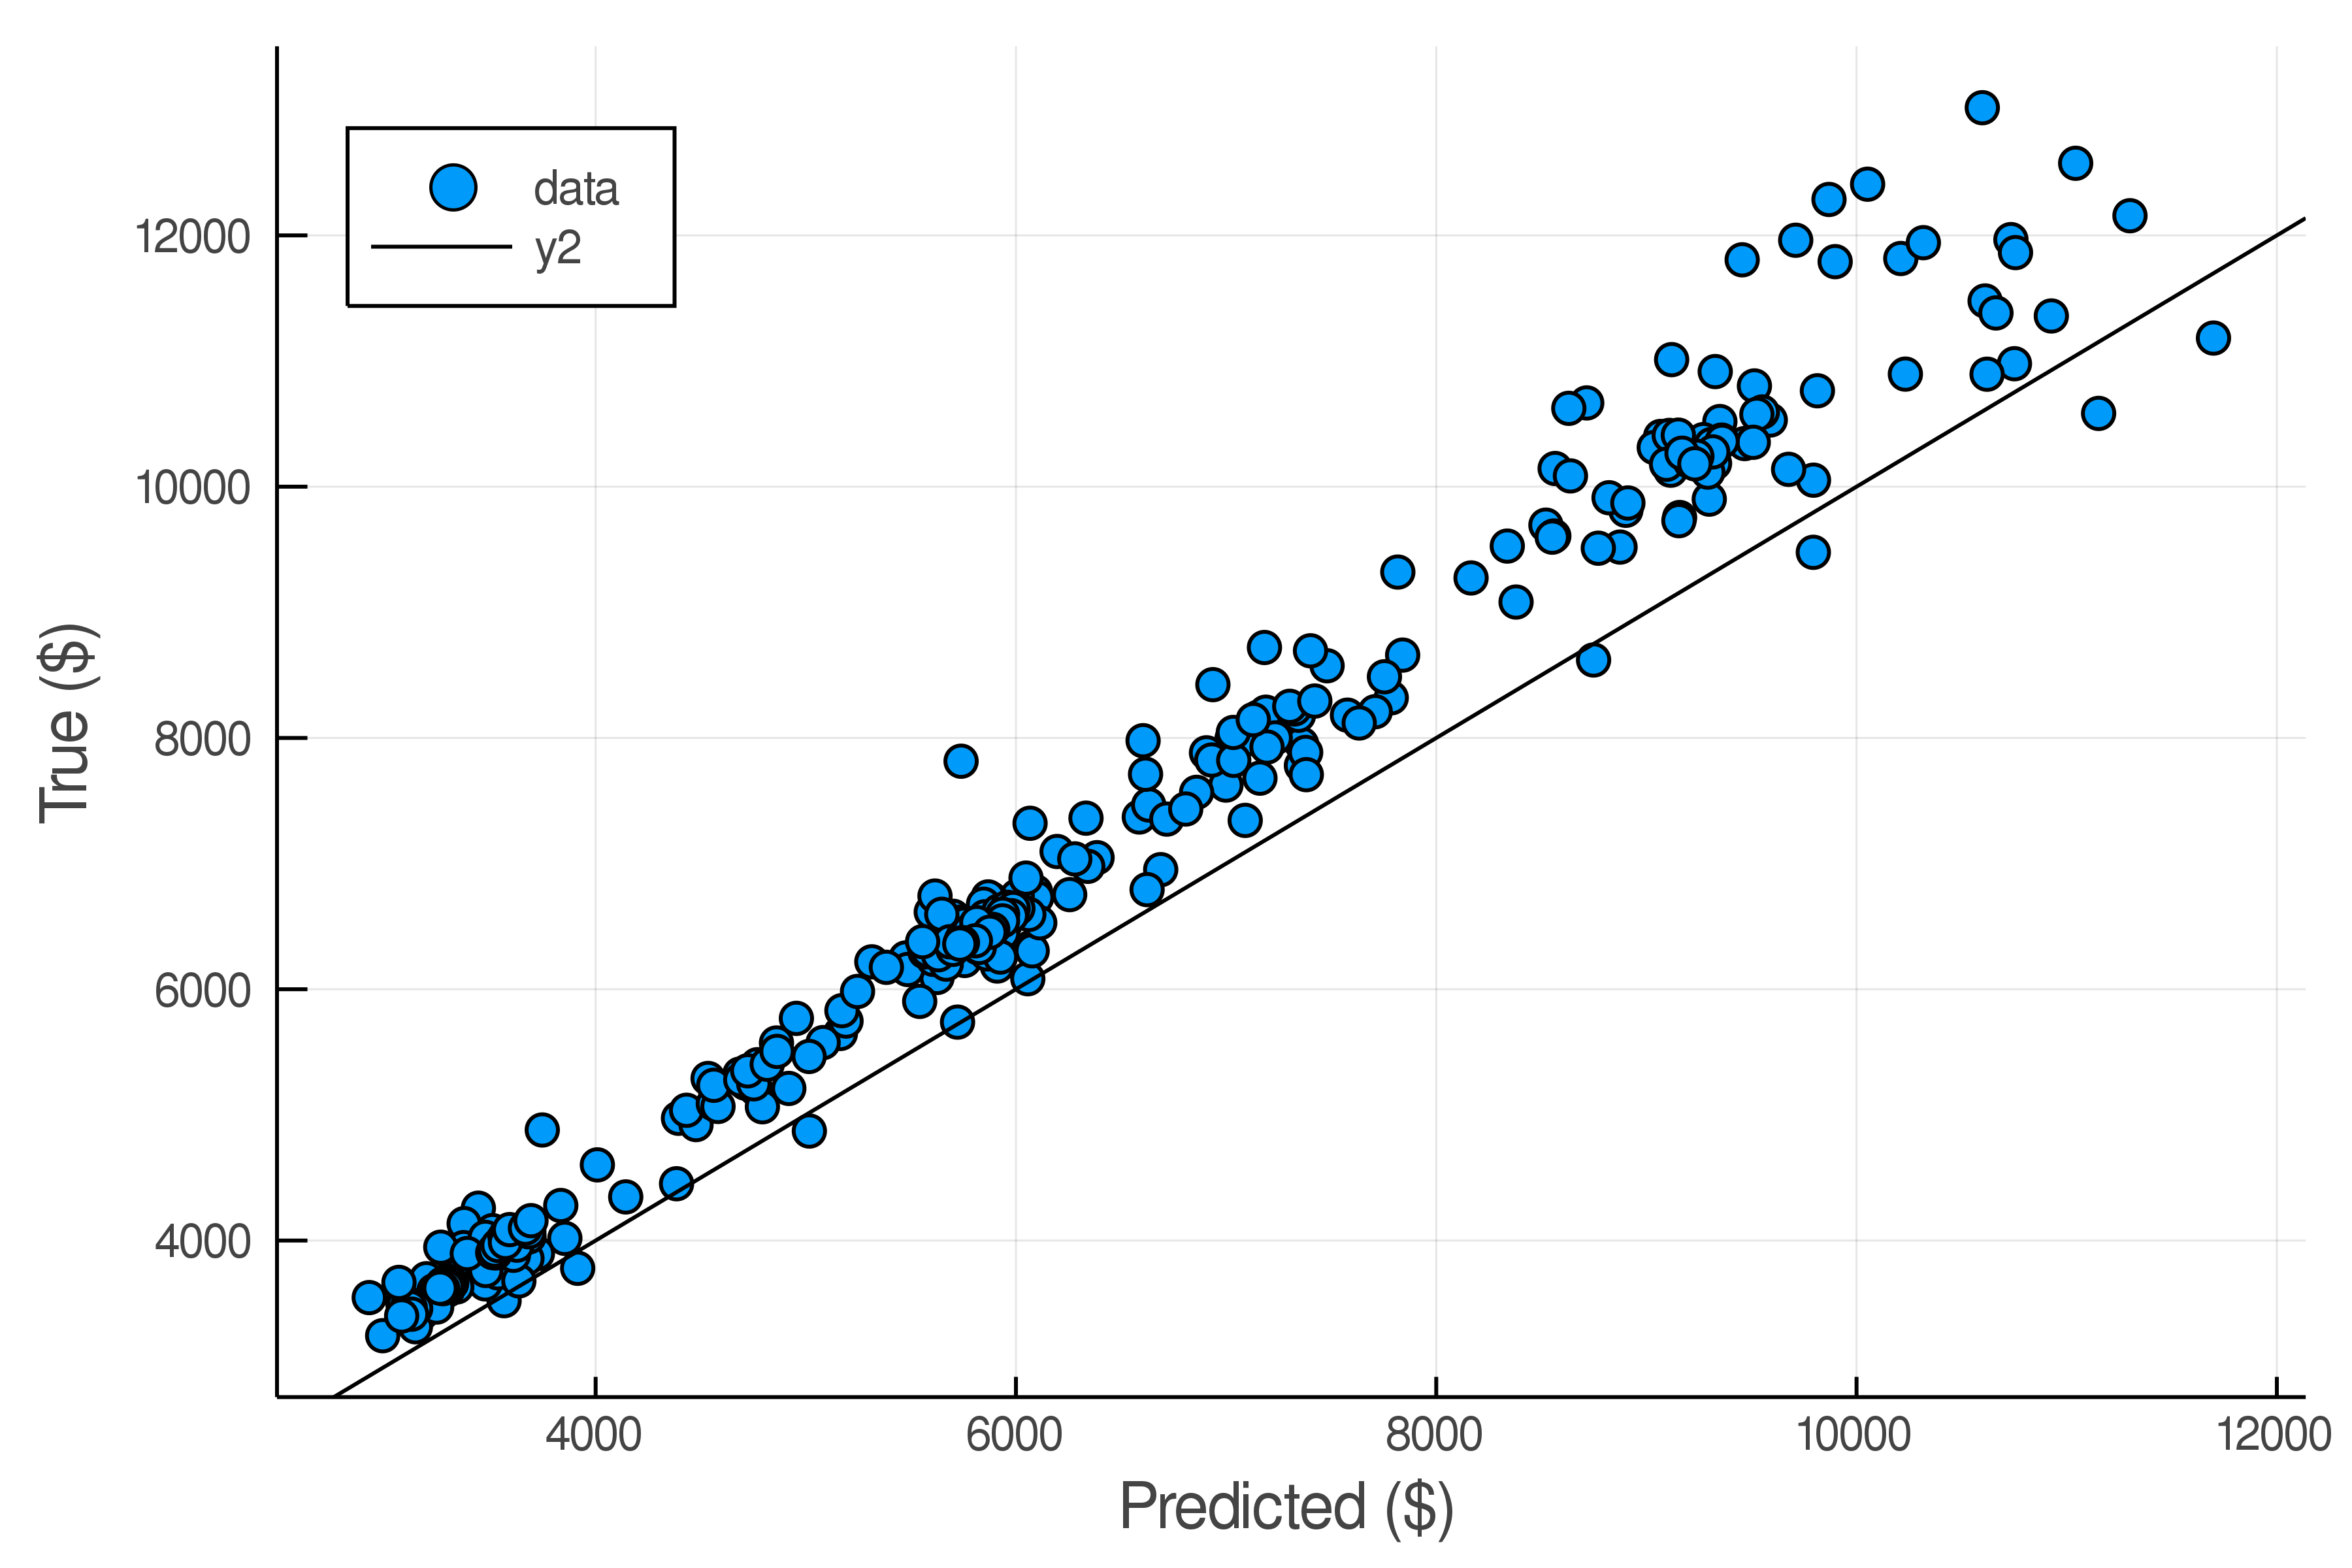
\includegraphics[width=.8\linewidth]{quantile_reg_price.png}
\caption{Regression for bitcoin pricing at the 5th quantile.}
\label{quantile_reg_price}
\end{figure}

At first glance it seems as though we have found a model that fits our data set fairly well. Given that we have 1617 total data points and 6 explanatory variables, we believe we face an issue of under-fitting with our model. We plan to bridge this gap with the addition of new features, more specifically, we consider making the return rate of bitcoin price as a quantity to predict. The return rate basically reflects the price variation during a short term, and that is of great interest because one can utilize it to predict his/her real-time gain when holding the bitcoin. 

Thus, the problem could be a classification problem, and we can use logistic loss function to predict the sign of the return rate in a probabilistic manner. As long as the model is believed to have a more than $50\%$ accuracy, the model is nontrivial, in the long run. Also, as a classification problem, it is easier for us to analyze the generalization properties of the model quantitatively.

\section{Exploration of Model Improvements}
Our initial thoughts coming into this project was that there should not be an analysis that allows for prediction of bitcoin prices with a significant probability, or else we would quit writing this paper and take the road to riches and fame. Thus we did not expect to find the statistically significant coefficients in our preliminary regressions analysis (Table \ref{BTC_Price_reg_analysis}). We also found relatively meaningful correlations between our explanatory variables and bitcoin price (Figure \ref{corr}).

\begin{table}[h]
\centering
\caption{Bitcoin Price Regression Analysis}
\label{BTC_Price_reg_analysis}
\begin{tabular}{@{\extracolsep{0pt}}lcccl} 
\hline
\hline
& Coefficients  & Std. Error  & t-Stat  & P-value\\ 
\hline
Intercept  & -32702.30093 & 1276.39136 & -25.62090 & 1.026e-121\\
GSPC price & 7.59396 & 0.39687 & 19.13449 & 1.0641e-73\\
NVDA price & 22.79817 & 1.46992 & 15.50978 & 1.1397e-50\\
Gold price & 10.75016 & 0.54272 & 19.80789 & 2.5468e-78\\
US infl. rate & 135775.16460 & 21258.24088 & 6.38694 & 2.2092e-10\\
3m. LIBOR & -219979.59714 & 16190.27047 & -13.58715 & 6.8992e-40\\
VIX & 162.67443 & 13.39684 & 12.14297 & 1.5753e-32\\
\hline
\multicolumn{2}{c}{\textit{Model results}}\\
\cline{1-2}
R Square & 0.79317 \\
Adj. R Sq. & 0.79240 \\
Std. Error & 1686.31682 \\
Observ. & 1617 \\
\hline
\end{tabular}
\end{table}

Given both a robust adjusted R squared metric and statistically meaningful explanatory variables, we expected our first model to predict out of sample points with a lower error than what was measured. After further research, we expect that some of the error and some of the misleading correlation coefficients were due to the non-stationarity of bitcoin pricing. 

Time series data is stationary if the mean and variance of a time series is constant throughout the series. Non-stationary data are by definition unpredictable and can lead to spurious correlation and unreliable statistical inferences \cite{ADFTesting}.

We tested the stationarity of bitcoin pricing using the Augmented Dickey Fuller test and found that our data set indeed failed to reject the null hypothesis that the underlying data set is non-stationary at the $95\%$ confidence level given that our p-value was $0.569257$ (see Table \ref{ADF_results_BTC_price}). We implemented this test in python using the statsmodels.tsa.stattools.adfuller package.\\

\begin{table}[h]
\centering
\caption{Augmented Dicky Fuller Results - Bitcoin Price}
\label{ADF_results_BTC_price}
\begin{tabular}{@{\extracolsep{8pt}}ll} 
\hline
\hline
                     & values     \\ 
\hline
Test Statistic       & -1.427018  \\
P-value              & 0.569257   \\
Critical Value(1\%)  & -3.434462  \\
Critical Value(5\%)  & -2.863356  \\
Critical Value(10\%) & -2.567737  \\
\hline
\end{tabular}
\end{table}

\noindent Test for unit root:
\begin{center}
    $\Delta y_t = \alpha + \beta t + \gamma y_{t-1} + \delta_1\Delta y_{t-1} + \delta_{\rho - 1}\Delta y_{t- \rho +1} + \varepsilon_t$\\
\end{center}

\noindent where:\\
\noindent $\alpha$ is a constant\\
\noindent $\beta$ is the coefficient on a time trend\\
\noindent $\rho$ is the lag order of the auto-regressive process\\
\noindent Null hypothesis:\\
\noindent $\mu_o$: $\gamma$ = 0 i.e unit root is present in the time series data and therefore exhibits non-stationarity.\\
Alternative hypothesis: $\mu_a$: $\gamma$ < 0 i.e there is no unit root present and the data is stationary.\\

After confirming our belief that bitcoin prices were non-stationary, we then used the transformation of the time series in order to calculate the log return of bitcoin prices. We chose the logarithm of bitcoin returns as this inherently adds a trend variable into the time series as we calculate daily returns as $\ln{\frac{today's price}{yesterday's price}}$. We performed the Augmented Dickey Fuller test using log returns (Figure \ref{fig_ADF_results_BTC_log_return}) and were able to reject the null hypothesis that the underlying data set is non-stationary with 95\% confidence (Table \ref{table_ADF_results_BTC_log_return}). 

\begin{figure}[h]
\centering
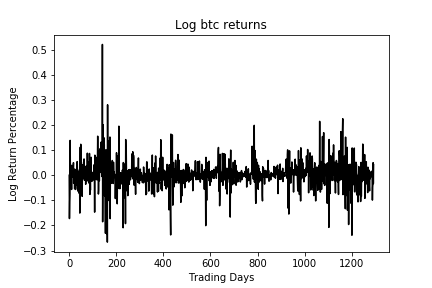
\includegraphics[width=0.85\linewidth]{btc_ret_1.png}
\caption{Augmented Dickey Fuller Test for log bitcoin returns where the x-axis is trading days starting at April 30, 2013.}
\label{fig_ADF_results_BTC_log_return}
\end{figure}

\begin{table}[h]
\centering
\caption{Augmented Dicky Fuller Results - Bitcoin Log Returns}
\label{table_ADF_results_BTC_log_return}
\begin{tabular}{ll} 
\hline
\hline
                     & values         \\ 
\hline
Test Statistic       & -8.746902e+00  \\
P-value              & 2.906225e-14   \\
Critical Value(1\%)  & -3.435465e+00  \\
Critical Value(5\%)  & -2.863799e+00  \\
Critical Value(10\%) & -2.567973e+00  \\
\hline
\end{tabular}
\end{table}

Following this, we used the logarithm of daily returns for all of our assets that were price measured which includes GSPC, NVDA, and gold. We then re-ran our regression to predict the transformed returns of bitcoin as well as a correlation analysis among our transformed explanatory variables and found significantly different results as seen in Table \ref{BTC_log_return_reg_analysis}. 

\begin{table}[h]
\centering
\caption{Bitcoin Log Return Regression Analysis}
\label{BTC_log_return_reg_analysis}
\begin{tabular}{lcccl} 
\hline
\hline
& Coefficients & Std. Error & t-Stat & P-value\\
\hline
Intercept & -0.02221 & 0.01286 & -1.72671 & 0.08441\\
GSPC return & -0.31686 & 0.18619 & -1.70187 & 0.08897\\
NVDA return & 0.12992 & 0.06167 & 2.10674 & 0.03529\\
Gold return & 0.25002 & 0.14688 & 1.70218 & 0.08891\\
U.S infl. rate & -0.36066 & 0.53897 & -0.66915 & 0.50350\\
3m. LIBOR & -0.02745 & 0.14524 & -0.18902 & 0.85010\\
VIX & -0.00085 & 0.00035 & -2.40127 & 0.01645  \\
\hline
\multicolumn{2}{c}{\textit{Model results}}\\
\cline{1-2}
R Square & 0.00816 \\
Adj. R Sq. & 0.00447 \\
Std. Error & 0.05116 \\
Observ. & 1617 \\
\hline
\end{tabular}
\end{table}

While these results differ from what was seen before, this matches our expectations that predicting future bitcoin prices could not be "this easy". Given that firms spend millions of dollars on research and trading each year, there was little belief amongst our group that something as simple as this regression could be of much value. Although many of these coefficients are no longer statistically significant from zero, we decided to keep them in the model as we believe each is justified by economic reason.

\section{Bitcoin Log Return and Problem Re-formalization}

As discussed above, the daily log return is of great interest because it reflects the price variation during a short term and one can use it to predict his/her real-time gain when holding the bitcoin. Even the exact quantity of the return can be trivial: we can focus on its sign, say, if the bitcoin price increase or decrease the next day. But here, we will construct our method so that our model will not only consider the sign of the log return, but also take into consideration the magnitude of the log return.

The distribution of the bitcoin log return is shown in Figure \ref{distribution_log_return}, together with its statistics. It is clear that the log return is sufficiently normally distributed. We thus classify the bitcoin log returns into four classes: large positive ($\geq \mu + \sigma$), positive ($\leq \mu + \sigma$ \&\& $\geq \mu$), negative ($\geq \mu - \sigma$ \&\& $\leq \mu$), large negative ($\leq \mu - \sigma$), i.e. class 0, 1, 2, 3 respectively. The percentages per class are shown in Table \ref{percent_per_class}.

\begin{figure}[h]
\centering
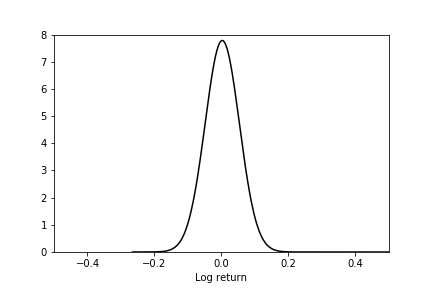
\includegraphics[width=.75\linewidth]{btc_ret_a.png}
\caption{Distribution of log transformed bitcoin returns. Statistics: $Mean = 0.002529$, $Min = -0.266198$, $Max = 0.520791$, $Std. = 0.051278$; $25\% percentile = -0.015508$, $50\% percentile = 0.001930$, $75\% percentile = 0.021883$}
\label{distribution_log_return}
\end{figure}

\begin{table}[h]
\centering
\caption{Percentages per Class:}
    % baseline accuracy:
    \begin{tabular}{lcccc}
    \hline
    \hline
    & \multicolumn{4}{c}{\textit{Classes:}}\\
    \cline{2-5}
    & 0 & 1 & 2 & 3 \\
    \hline
    percentage & 8.0\% & 38.1\% & 45.2\% & 8.7\% \\
    \hline
    \end{tabular}
    \label{percent_per_class}
\end{table}

Formally, we set the problem to be a multi-class classification problem. Our expectation is to maximize the confidence of classifying a point to its corresponding class.

\section{Predicting Bitcoin Log Return via Support Vector Classifier (SVC)}

We first employ the support vector machine (SVM) method to the classification problem, i.e. use support vector classifier (SVC). The SVC method works as follows:

Given training vectors $x_i \in \mathbb{R}^p$
, i=1,…, n, in two classes, and a vector $y \in \{1, -1\}^n$, SVC solves the following primal problem:
\[\min\limits_{w, b, \zeta} \frac{1}{2} w^T w + C \sum_{i=1}^{n} \zeta_i\]
\[\textrm {subject to } y_i (w^T \phi (x_i) + b) \geq 1 - \zeta_i,\]
\[\zeta_i \geq 0, i=1, ..., n\]
The decision function is:
\[\operatorname{sgn}(\sum_{i=1}^n y_i \alpha_i K(x_i, x) + \rho)\]

In this problem, we simply use lagged features introduced previously, with selection according to model performance. The $lag$ is set to be $1$, $2$, $3$, $4$, $5$ days, respectively. And we use the standard machine learning package scikit-learn to try to fit a multi-class classifier that can predict the bitcoin daily log return. The encoding scheme we are using is one-vs.-rest (OvR) via "sklearn.multiclass.OneVsRestClassifier". We also enable probability estimates for all of the following results. Scikit-learn also provides other several kernel functions, such as radial basis function, linear, polynomial, sigmoid, etc.

We analyze the effectiveness of the model by calculating for the confusion matrix via "sklearn.metrics.confusion\_matrix". By definition a confusion matrix $C$ is such that $C_{i,j}$ is equal to the number of observations known to be in group $i$ but predicted to be in group $j$. Thus, an ideal confusion matrix is a diagonal matrix. We normalize the confusion matrix to $C_{i,j}^{n}$ by:
\[ C_{i,j}^{n} = \frac{C_{i,j}}{\sum_{k=1}^{nc}C_{i,k}} \]
where $nc$ is the number of classes.

$C_{i,j}^{n}$ is the expectation of the probability of a point in class $i$ being classified as class $j$. Or formally:
\[
C_{i,j}^{n} = \mathbb{E}[P(y' \in class \: j \;|\; (y|x) \in class \: i)]
\]

In order for the model to be effective in the long run, we expect a more than $50\%$ accuracy for each of the classes. In fact, as a multi-class classifier, the baseline of the performance can be even lower than $50\%$.

\subsection*{The radial basis function (RBF) kernel}
We first use a radial basis function (RBF) kernel function as to save computational power. RBF calculates the local density of each class and use that to classify new points within the window. The normalized confusion matrix of the most promising RBF model for both training and testing are listed below:

\noindent  for $lag = 2$:
\smallskip\\
Variables: \textit{GSPC\_log\_ret}, \textit{BTC\_log\_ret}, \textit{NVDA\_log\_ret}, \textit{Gold\_log\_ret}. 4 variables, thus $4\times lag$ features.
\smallskip\\
Training:

\begin{center}
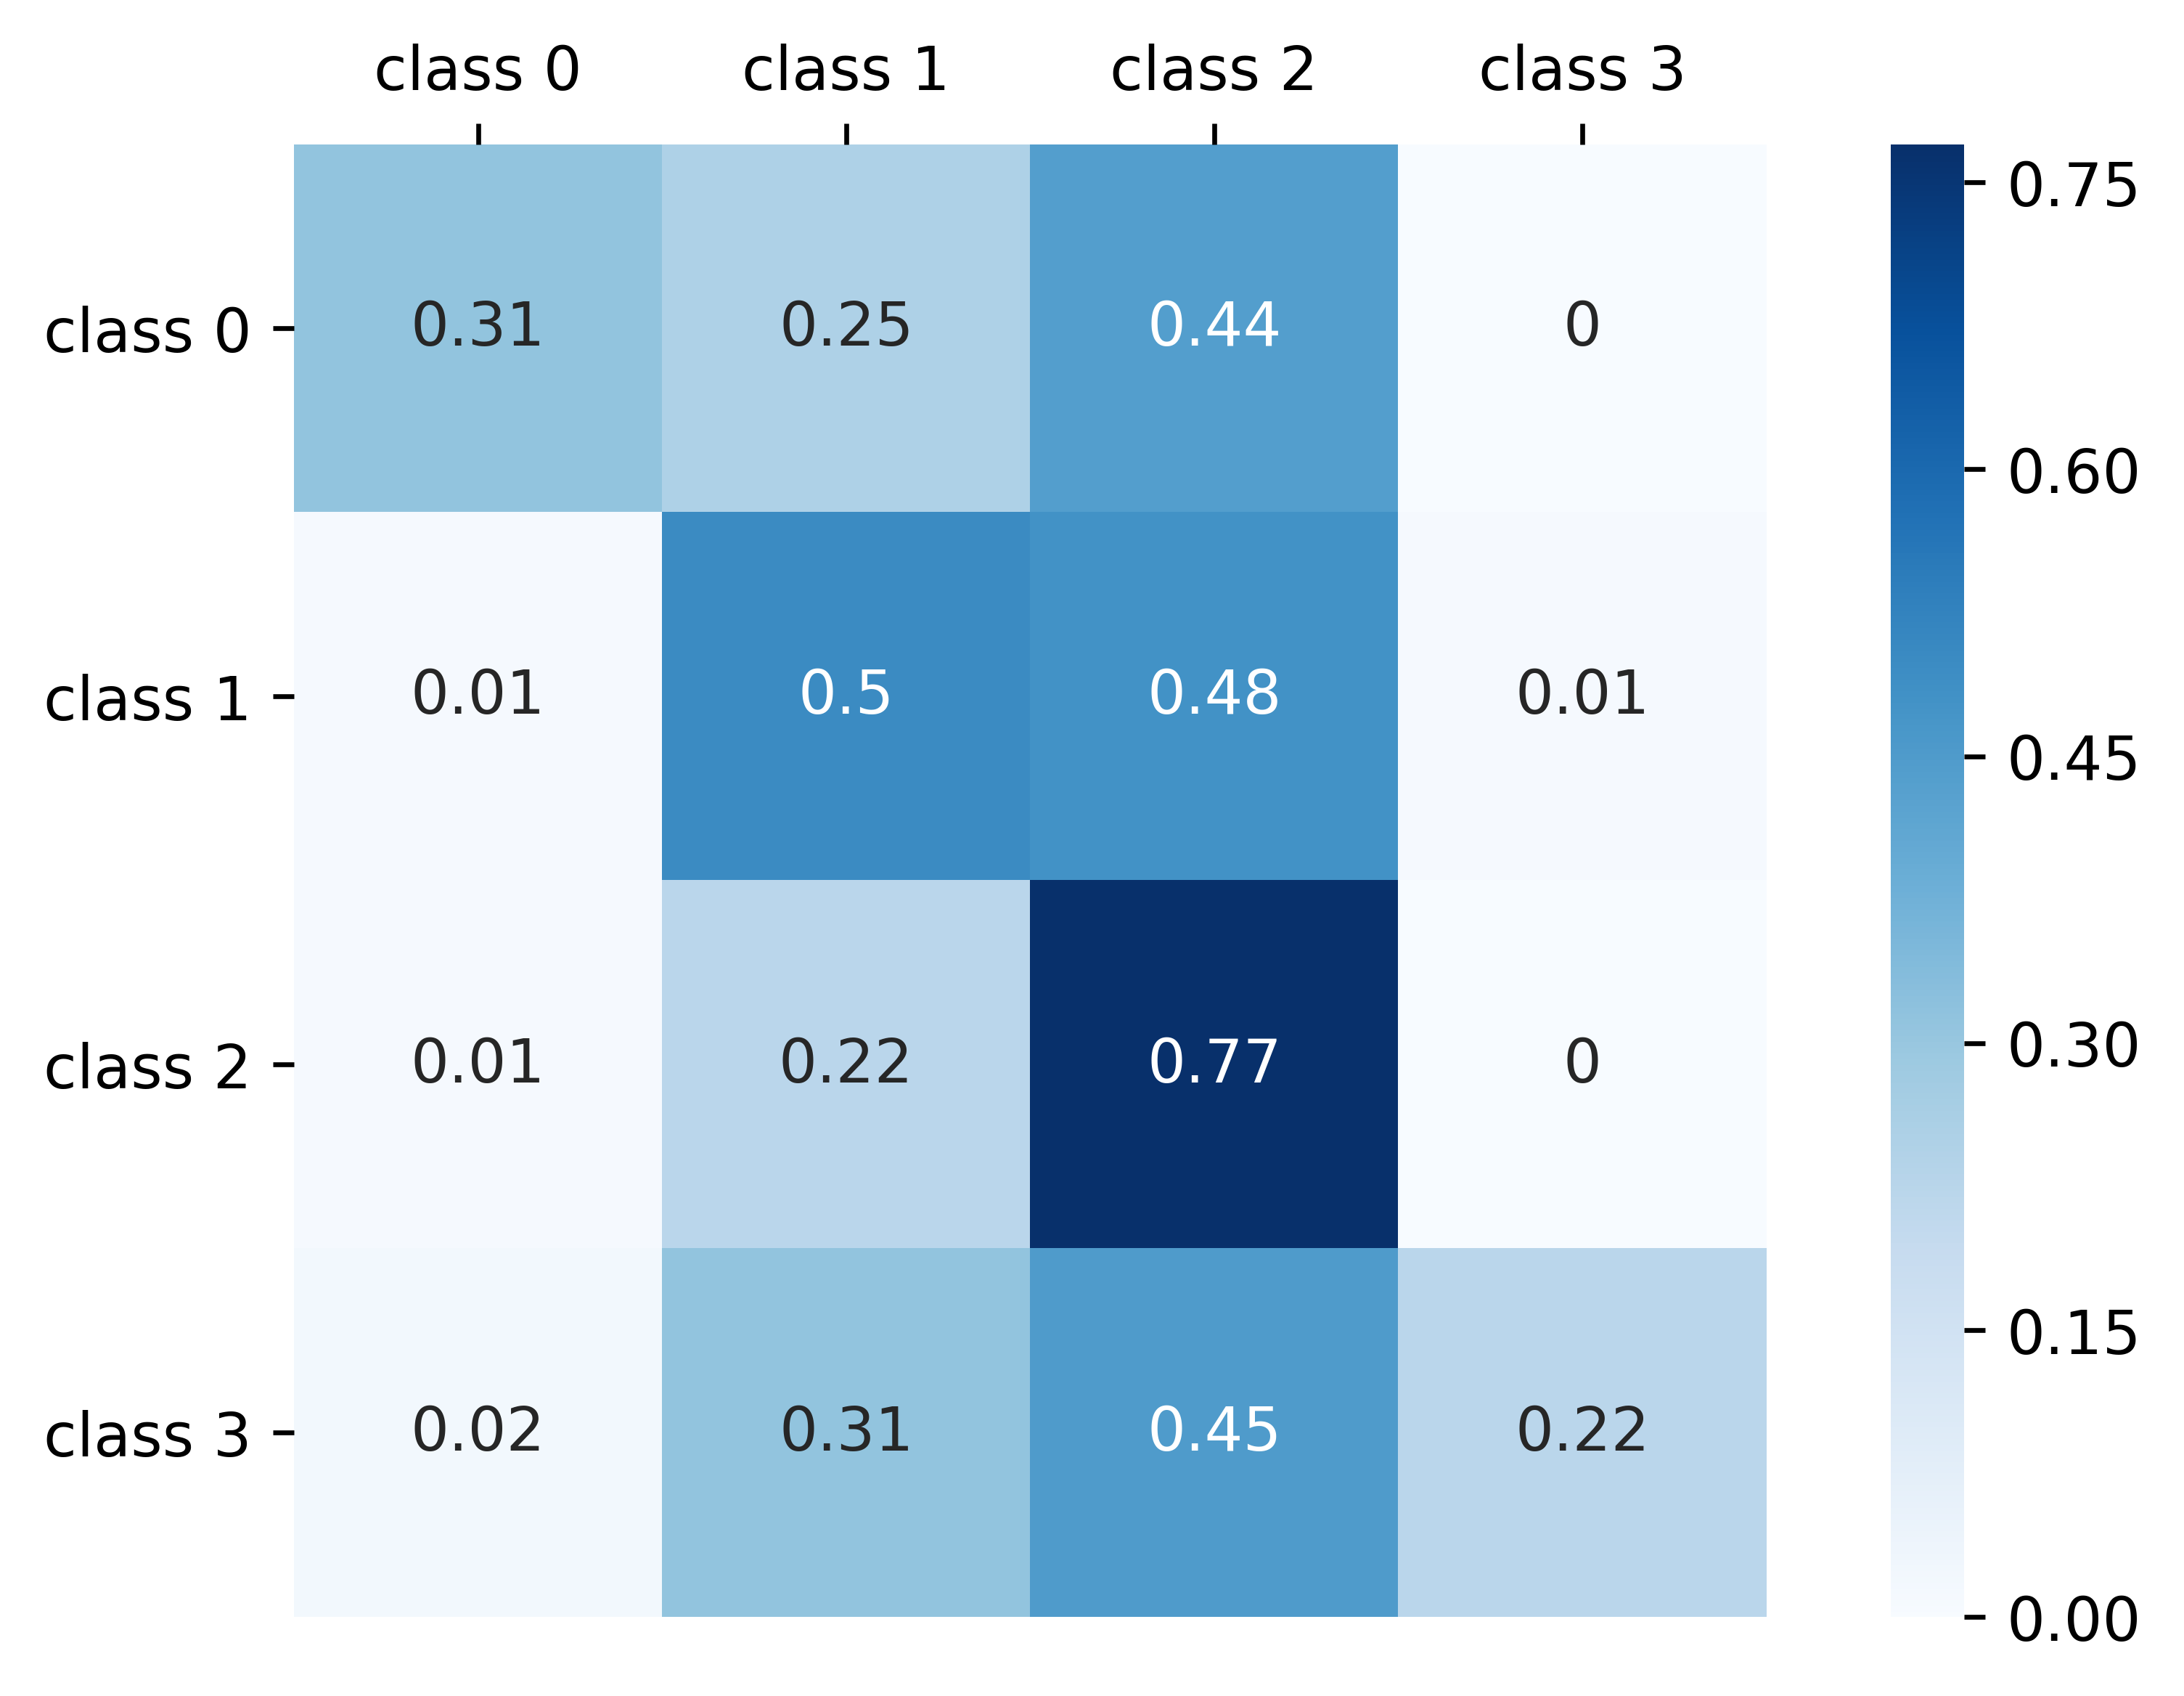
\includegraphics[scale=0.35]{train_cfs_mat_2_rbf.png}
\end{center}
Testing:

\begin{center}
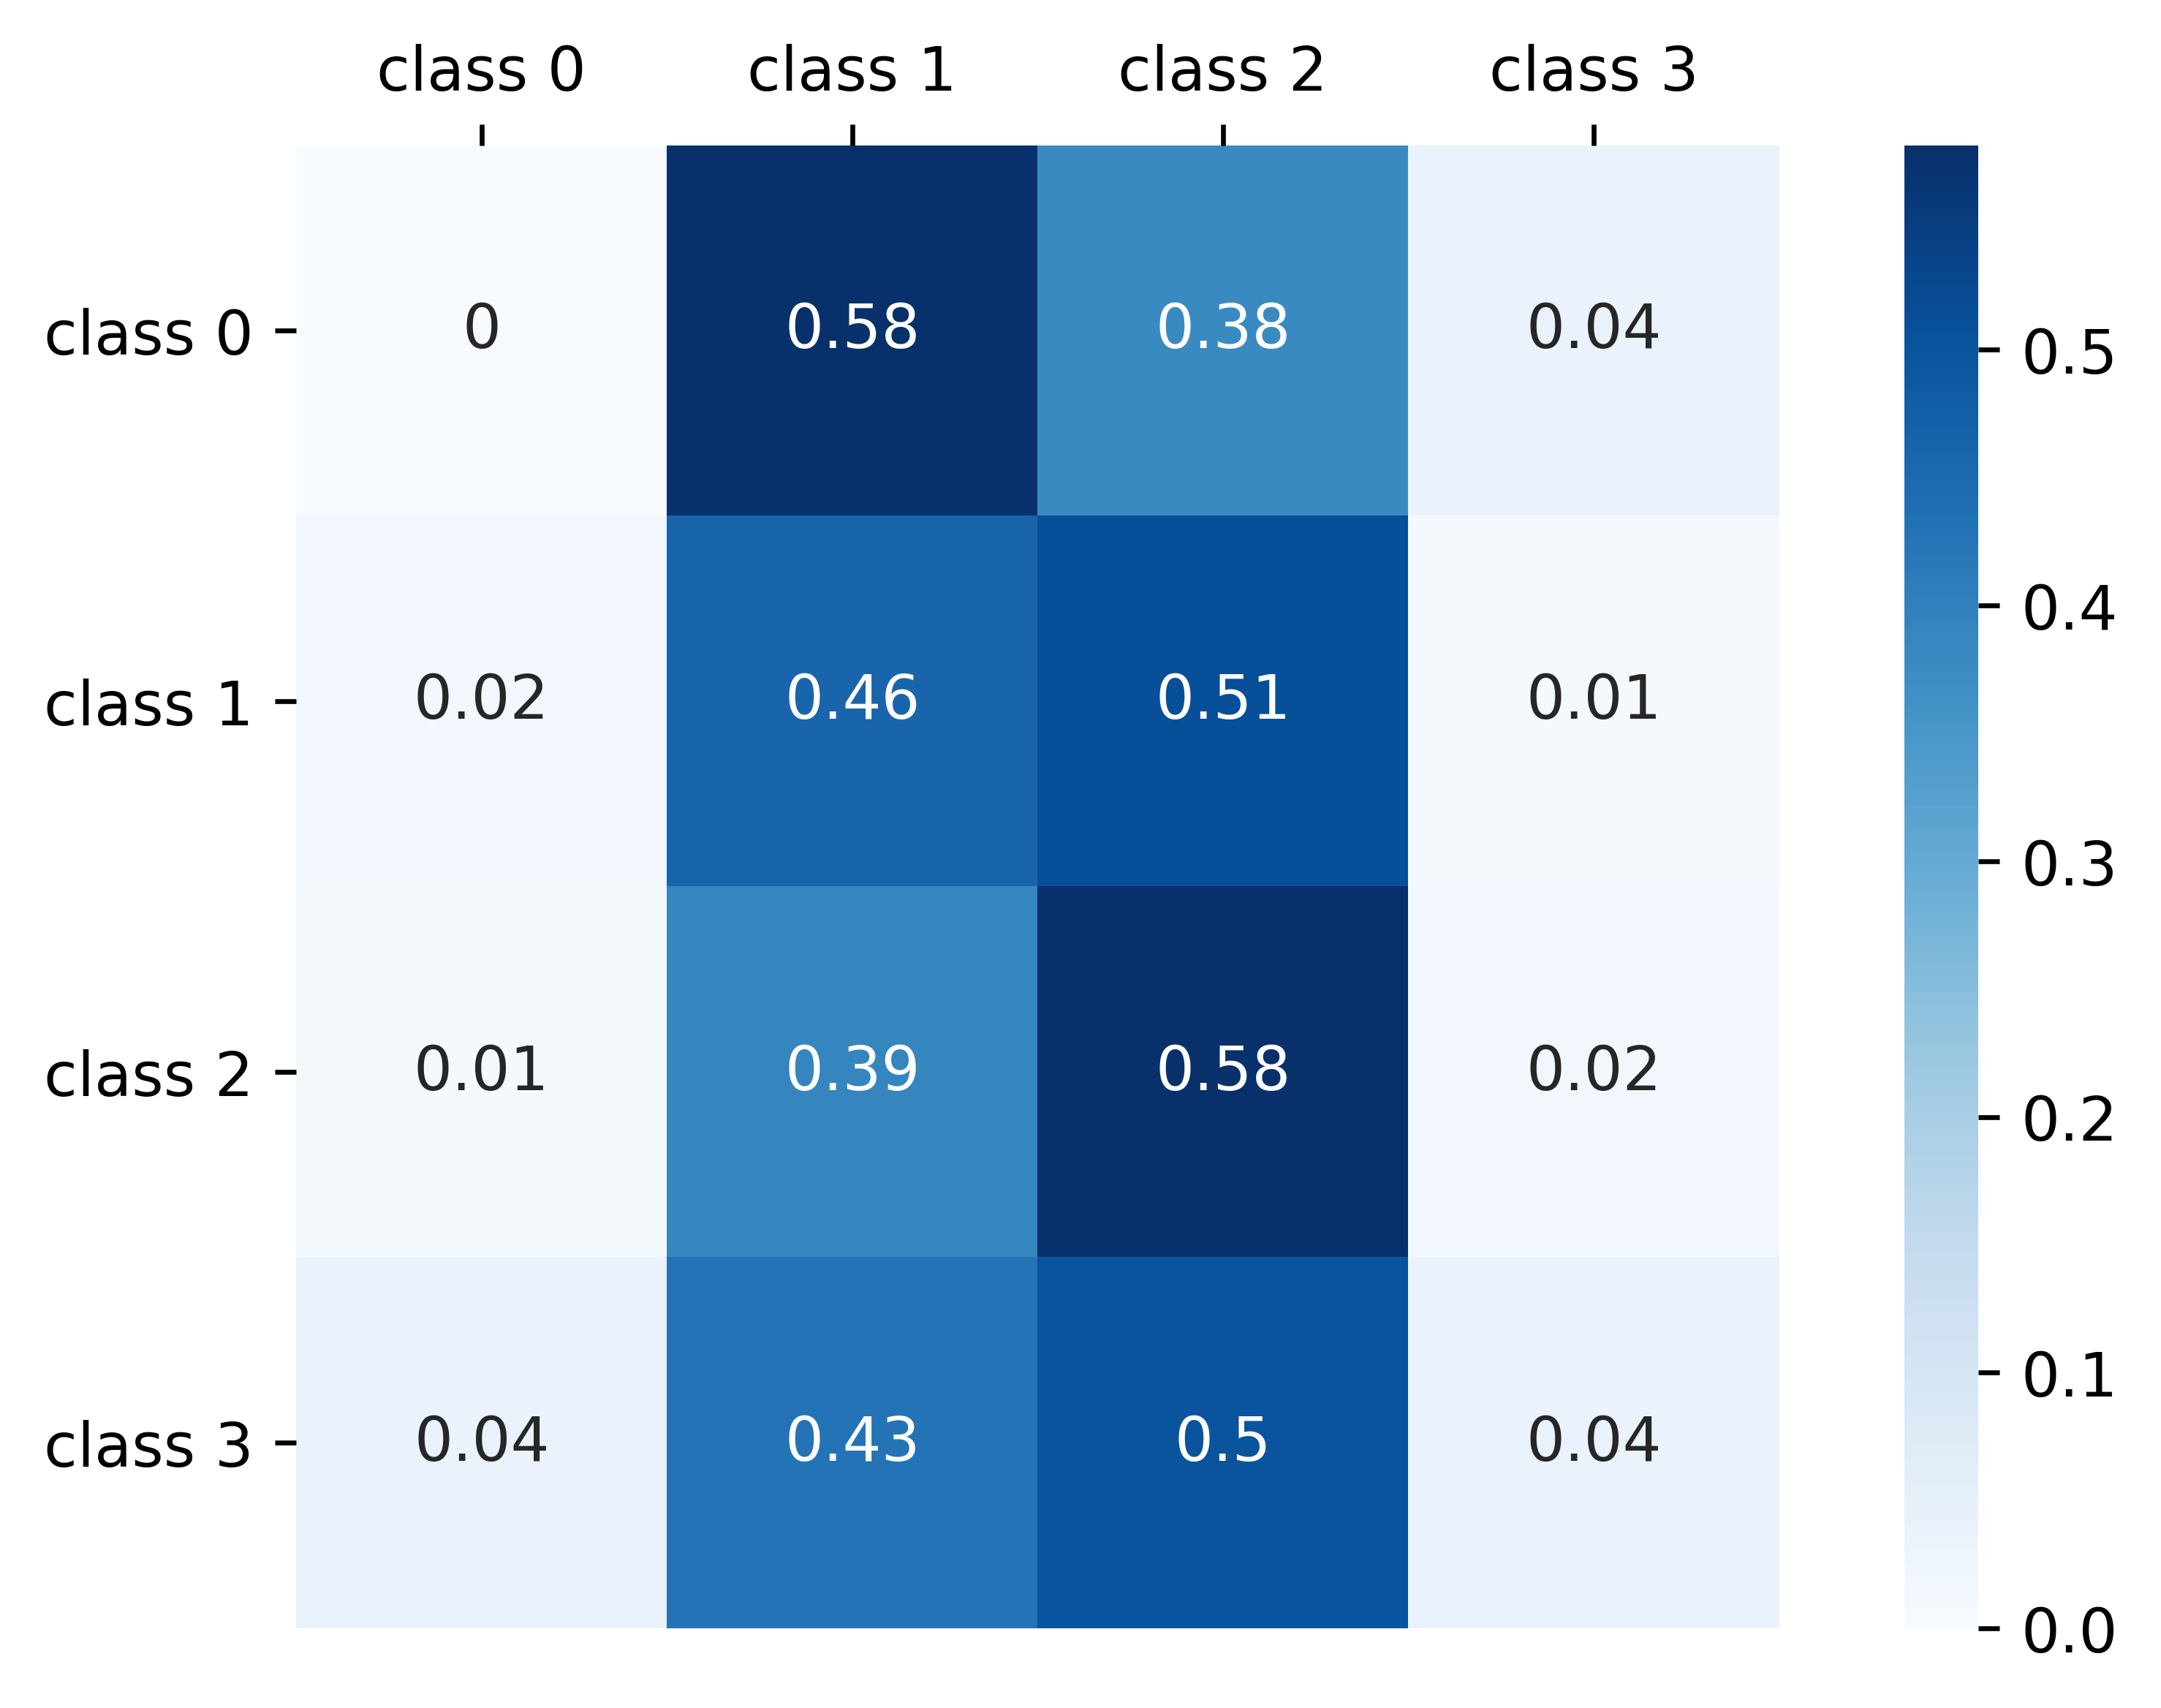
\includegraphics[scale=0.35]{test_cfs_mat_2_rbf.png}
\end{center}

The training process went smoothly. However, we end up with poor accuracy for class 0 and 3. Class 1 has $50\%$ accuracy, and class 2 shows the highest accuracy, $77\%$. In testing, we are having very poor predictive accuracy for class 0 and class 3. The accuracy for class 1 is just below $50\%$, while we have a over $50\%$ accuracy for class 2. \textbf{(This means our model for classifying class 2 is at least better than a random number generator)}. However, we don't have a significantly higher than $50\%$ test accuracy for class 2. So in real life, sadly, it is risky to apply this model to make any financial decisions.

One reason why our model fails to classify class 0 and 3 accurately is the insufficient examples of class 0 and 3. We only have tens of such large bitcoin price fluctuation in history. So our model may not borrow too much predictive power from those examples.

We also have tried adding/removing features in this case. We find that neither adding/removing variables help improve error. Adding $lag$ will instantly lower the training error but increase the test error, resulting in a typical over-fitting scenario. Decreasing $lag$ will instantly increase both the training and testing error, resulting in a under-fitting case. We can only hope that, at least for class 2, our model shows potential to generalize.

\subsection*{The polynomial kernel}
We use the polynomial kernel implemented in scikit-learn package. The polynomial kernel function basically does a further feature transformation by converting the current features into higher-order polynomials. Finding the exact order of the polynomial is done by the hidden algorithms, yet the fitting is still done in a SVM manner. We present the best model we can fit with polynomial kernel as follows:

\noindent  for $lag = 5$:
\smallskip\\
Variables: \textit{GSPC\_log\_ret}, \textit{BTC\_log\_ret}, \textit{NVDA\_log\_ret}, \textit{Gold\_log\_ret}, \textit{US\_inflation\_rate}, \textit{3\_month\_LIBOR}. 6 variables, thus $6\times lag$ features.
\smallskip\\
Training:

\begin{center}
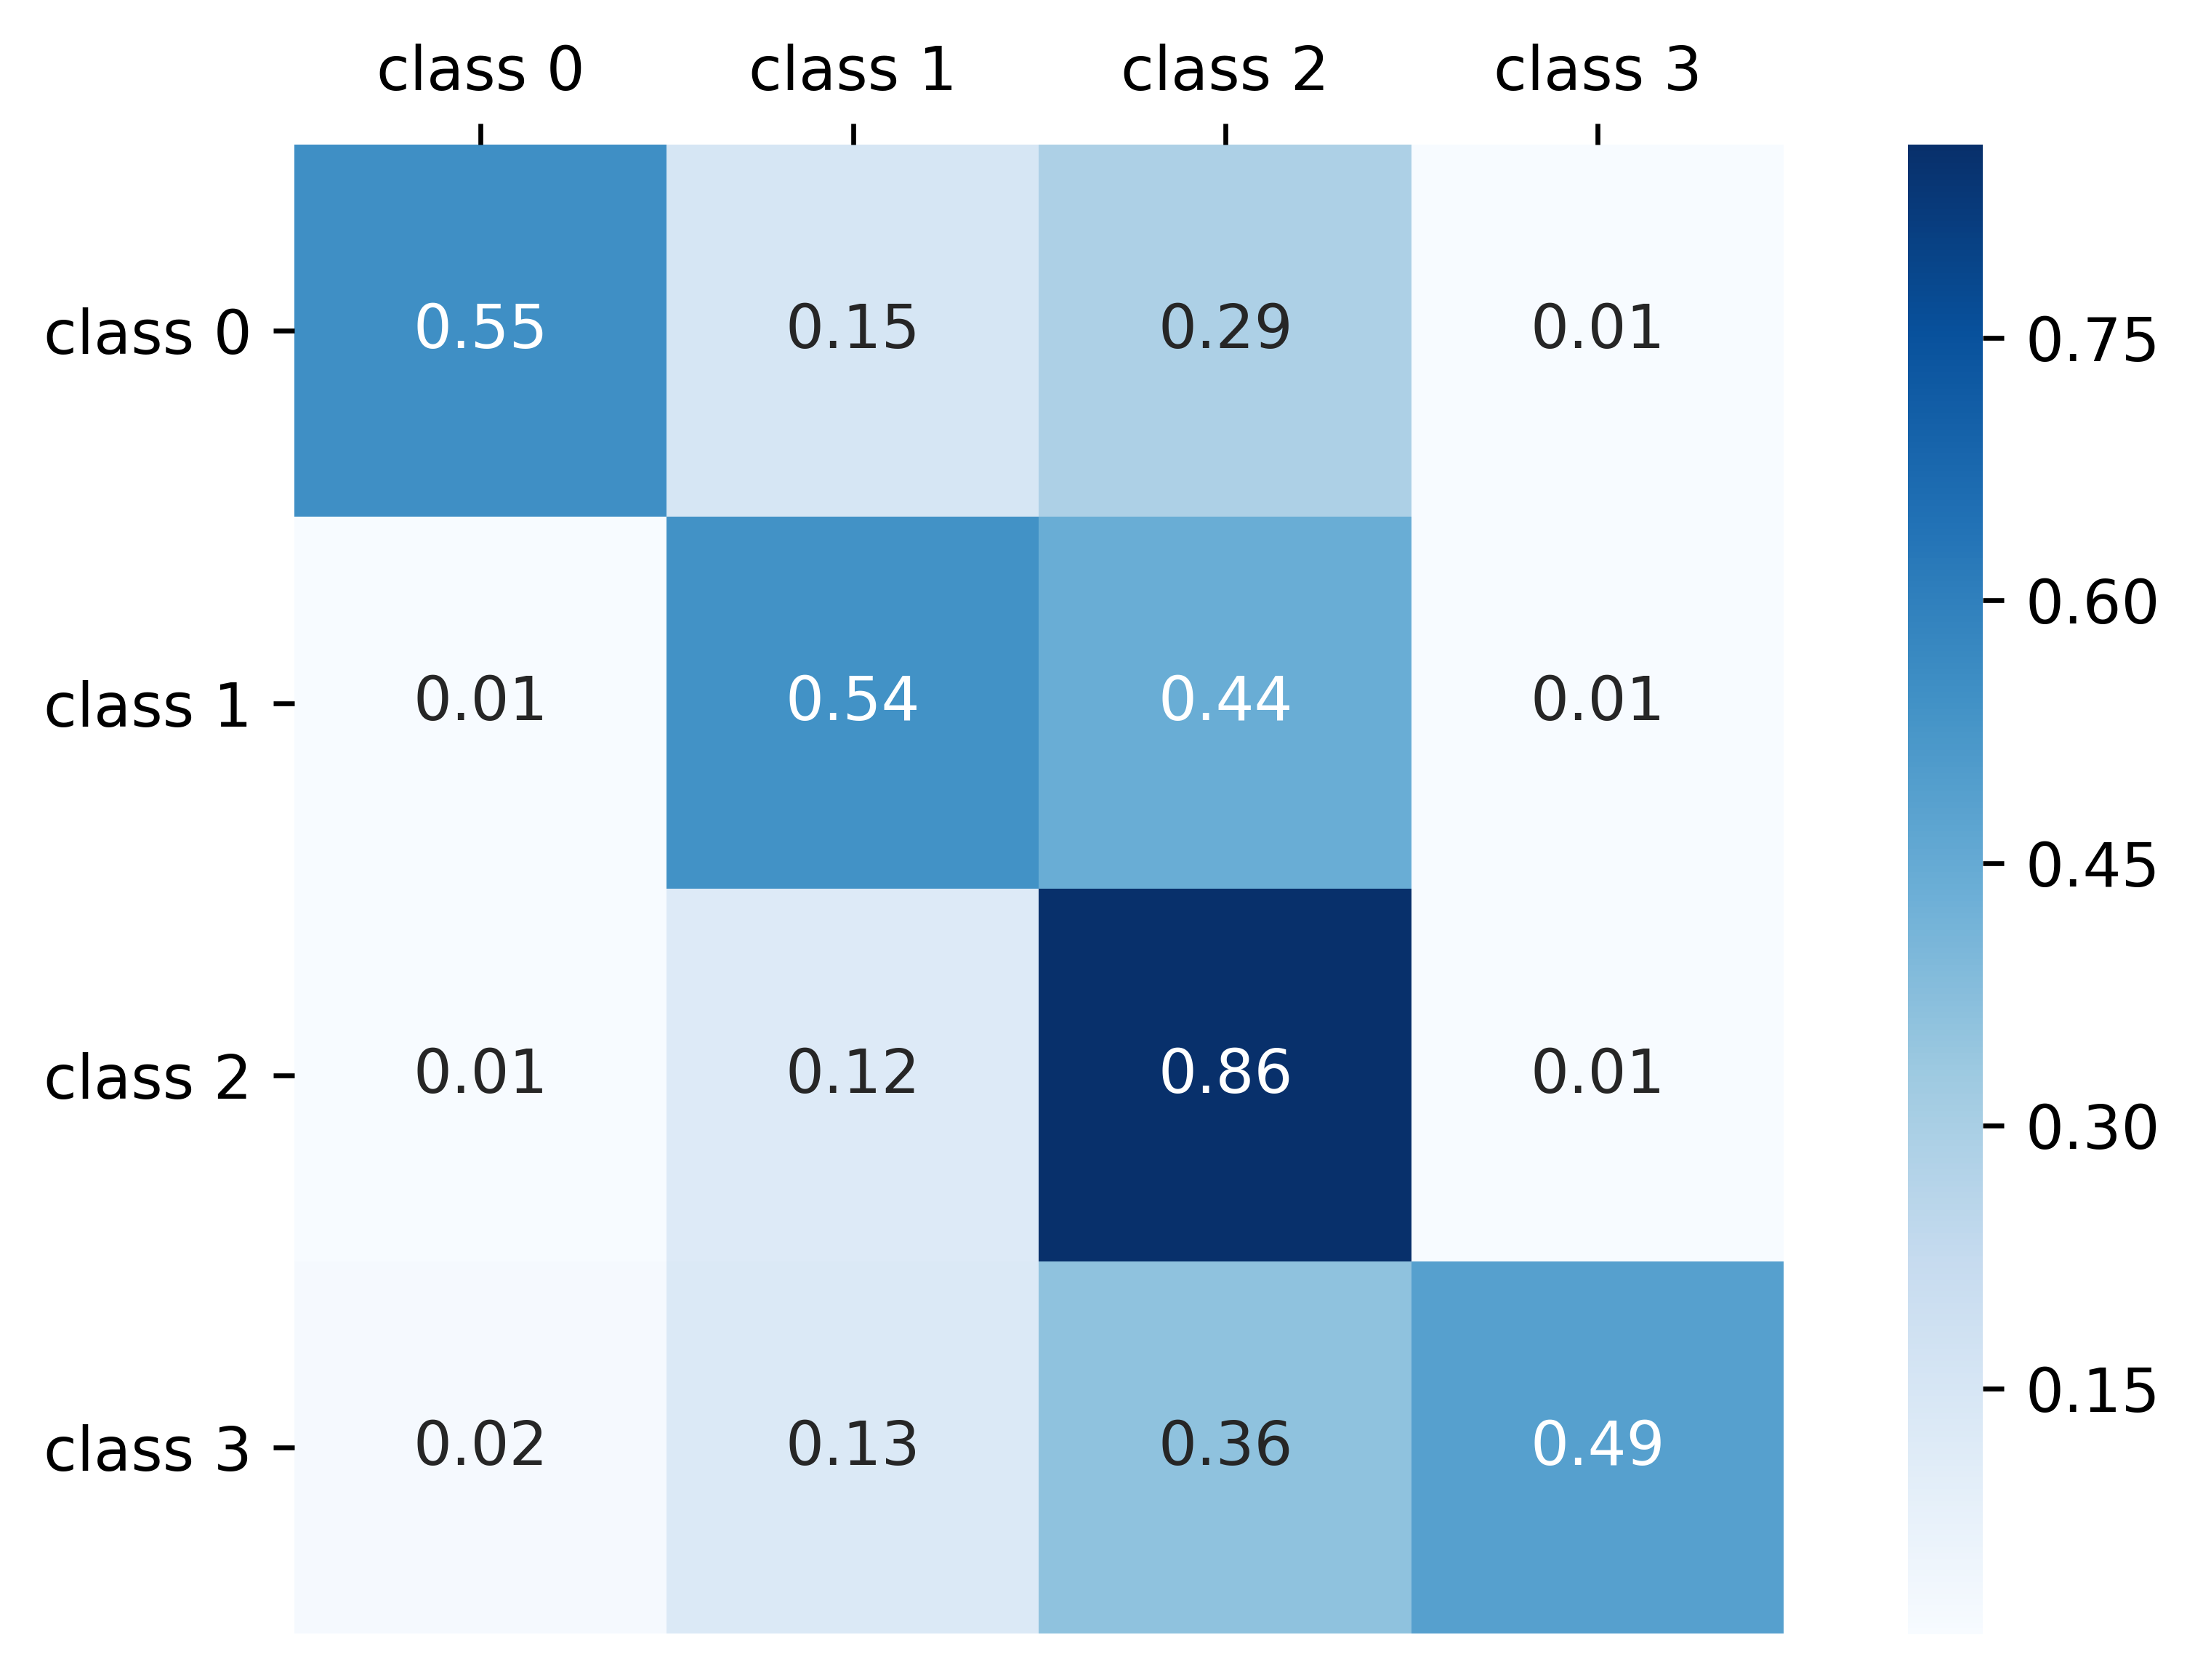
\includegraphics[scale=0.35]{train_cfs_mat_5_poly.png}
\end{center}
Testing:

\begin{center}
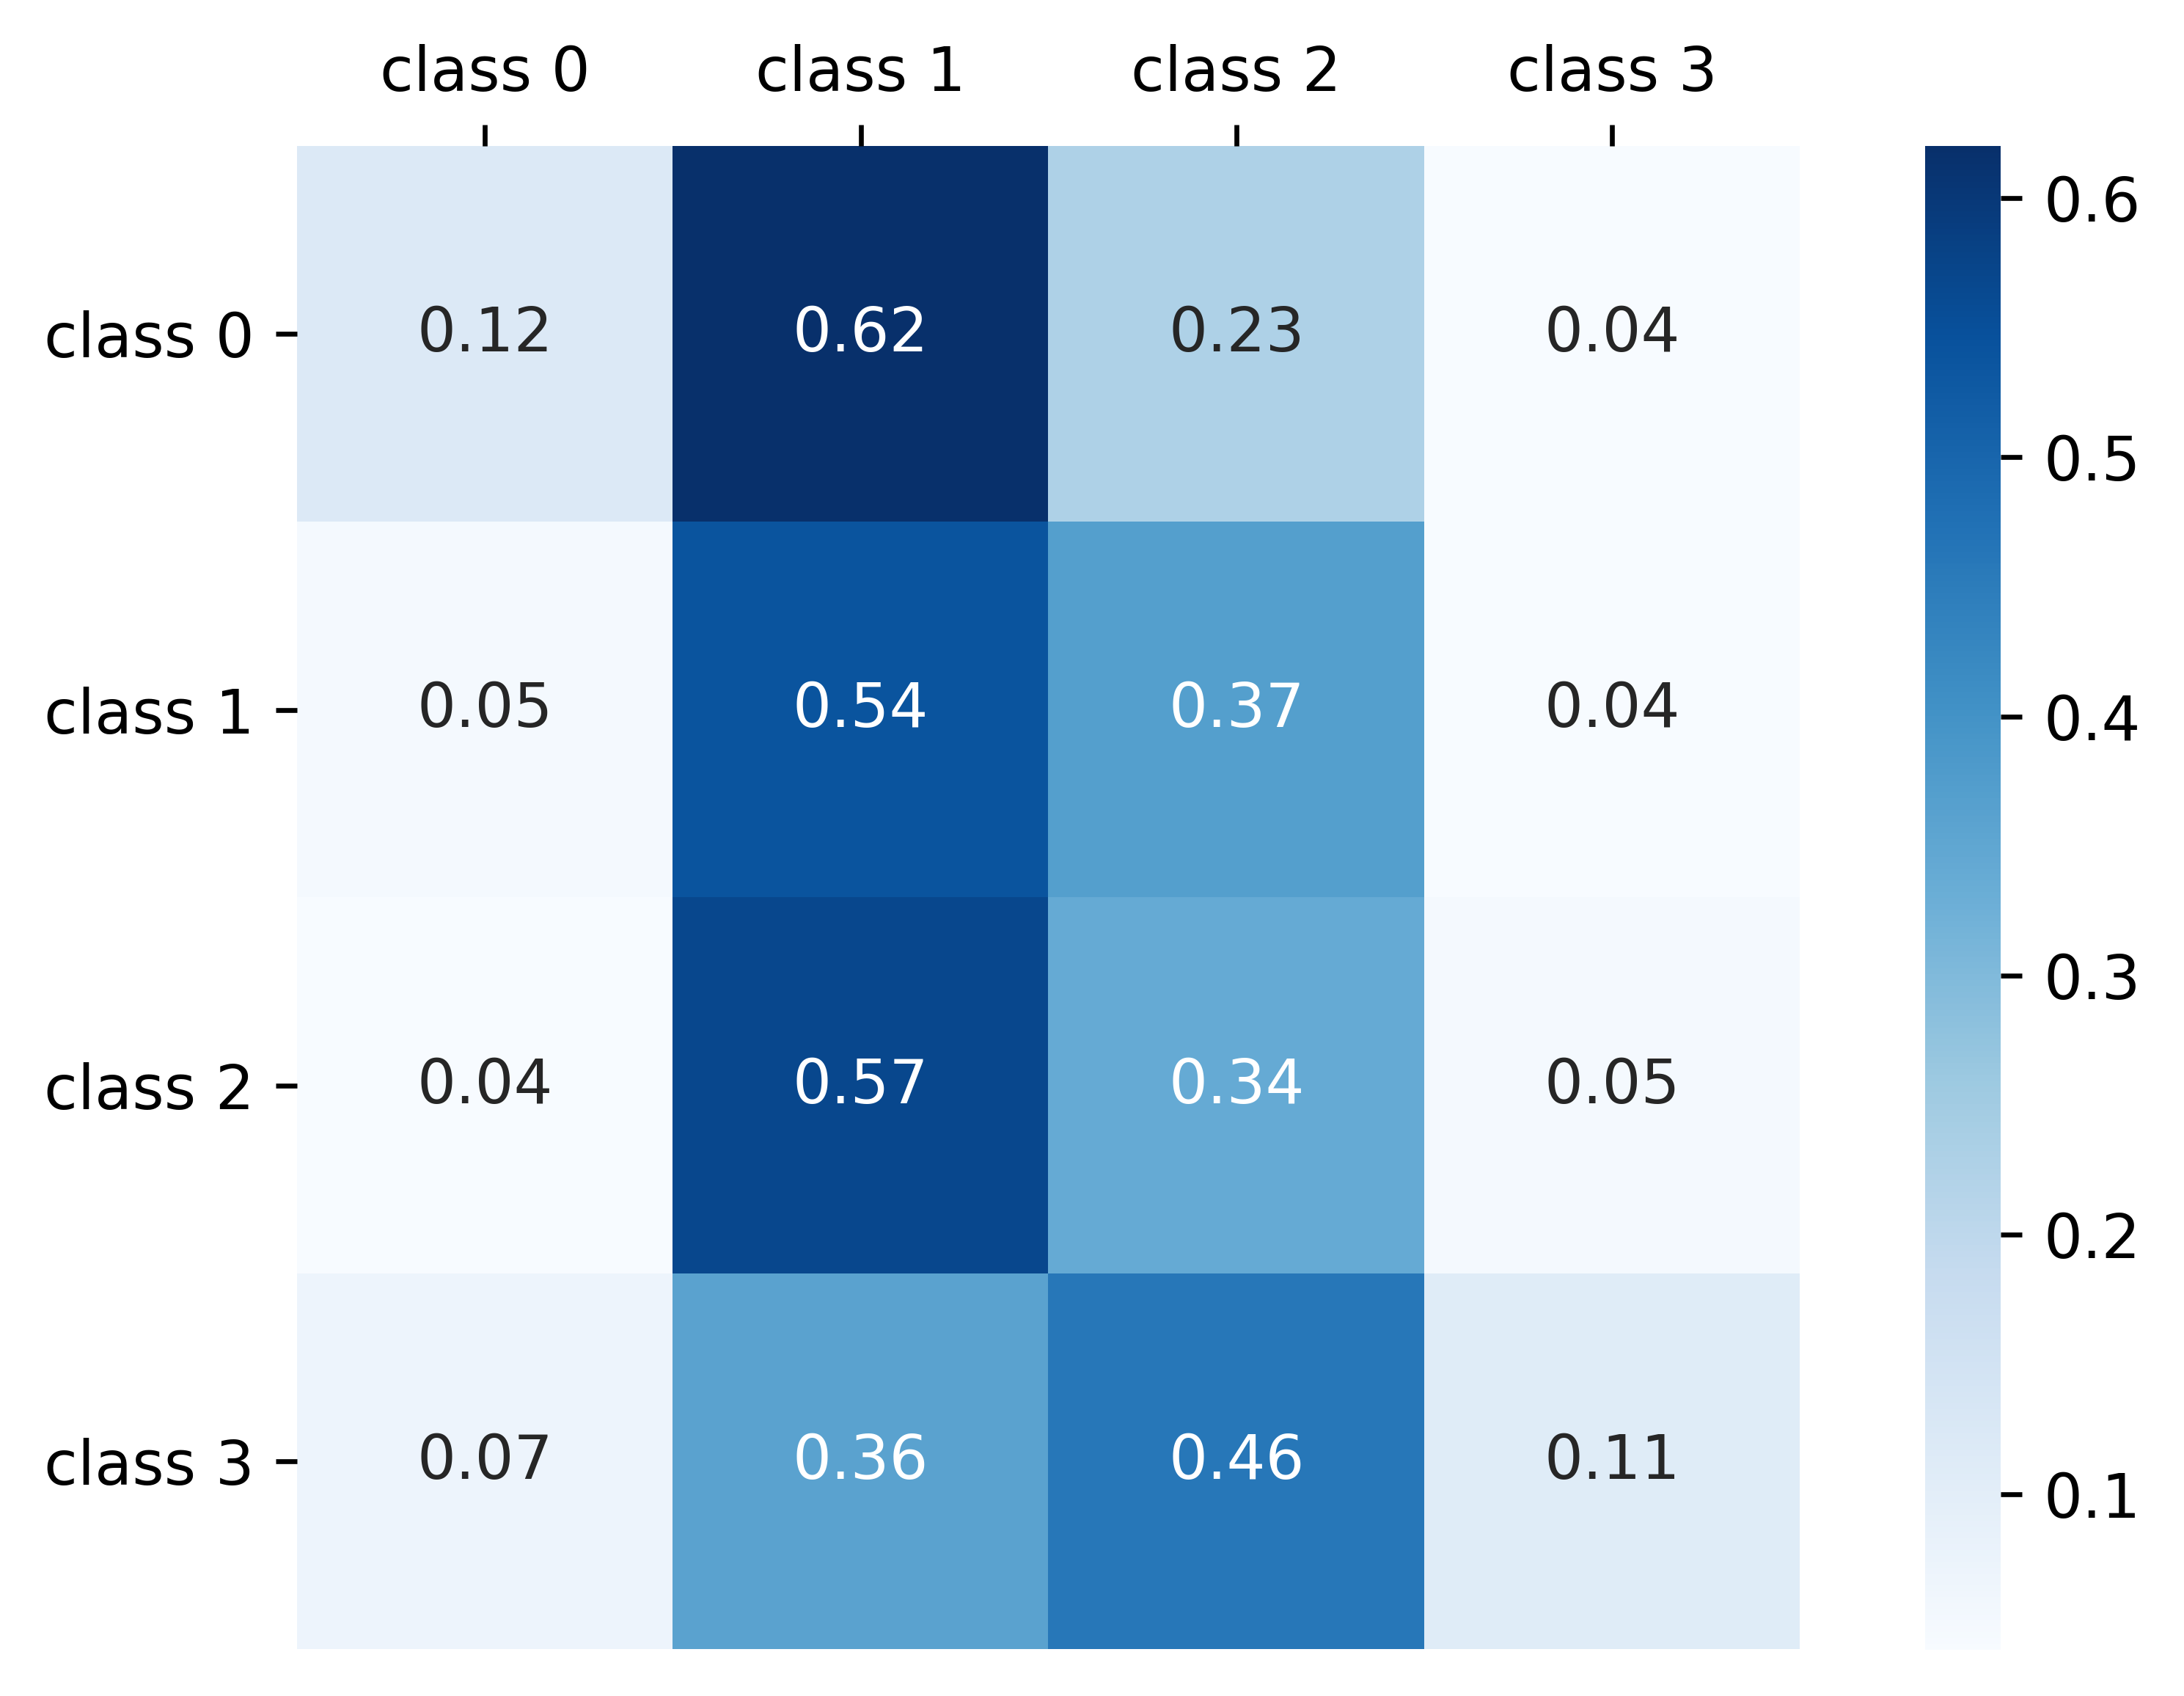
\includegraphics[scale=0.35]{test_cfs_mat_5_poly.png}
\end{center}

The polynomial kernel shows much more power in fitting the complex model. After training, we have a more diagonalized confusion matrix. \textbf{In fact}, if we keep adding $lag$'s, the training error will converge to $0$. However, over-fitting happens as expected. So we have to find the sweet point with an intermediate $lag$ and a reasonable test error.

However, even we did everything to find the sweet point of generalization, there is no clear sign the model generalizes. At the end, we have a test confusion matrix with poor predictive power. In both of the confusion matrices, we have the same $C_{i,i}^n$ for class 1. However, the model performs much worse than on the training set for the rest of the classes. Thus, it is very risky to generalize the classifier even for only the class 1, because the result could be simply a coincidence.

We have also tested the linear and sigmoid kernels, both of which are even worse than the two introduced above. Apparently most of the real world problems are non-linear, and the linear model cannot outperform the polynomial model on our data set. For the sigmoid kernel, the resulting confusion matrices are erroneously sparse: it classifies every point into class 2 or class 3. The analysis on those two kernels is beyond the scope of this report.

From the confusion matrices, we see that the SVM method does not perform well on this data set. However, we can discuss the results in the following dimensions: \textbf{1.} None of the models predict class 0 or class 3 points very well, that is, the model cannot predict the extreme values. This is probably due the the lack of data examples. \textbf{2.} The RBF model seems to be useful for differentiating class 2 points from other classes while the polynomial model shows potential in classifying class 1 points from others. This is significant because this means the model is effective in predicting, at least partially, the bitcoin log return. \textbf{3.} Again, in fact, as a multi-class classifier, the baseline of the performance is even lower than $50\%$. We still stand a chance in effectively classify the target data point with the combination of models, i.e., combining the prediction of the RBF and the polynomial model to make a comprehensive prediction. \textbf{4.} We have gathered 10 variables, with $lag$'s, we have a large variety of choices of features to use. However, for different models, the feature may improve one while damaging another. For example, smaller $lag$'s are appreciated in the RBF models, while larger $lag$'s can effectively improve the polynomial model. In reality, the market acts fast to some fluctuations, but some profound events will exert their impact gradually and slowly (e.g. The U.S.-China Trade War). Different models may have captured different aspects of the real world.

\section{Predicting Bitcoin Log Return via k-Nearest Neighbors (kNN)}

We then try to implement the classification starting with non-parametric method.

In the kNN algorithm, the training examples are represented as a vector in a multidimensional feature space, each with a class label. In the classification process, we define $k$ to be the amount of neighbours we want check for distribution. Given an unlabeled vector, we take its nearest $k$ neighbours, where distance is using Euclidean distance or Hamming distance for discrete variables. The vector will be assigned using the weights of its neighbours labels.

For the $i$th nearest neighbour is assigned with weight $w_{i}$, with $\sum_{i=1}^n w_{i} = 1$. For query $x$, it is defined as follows \cite{samworth2012optimal}:
\[
\scalemath{0.95}{
w_{i}=
\begin{cases}
\frac{d(x,x_{k})-d(x,x_{i})}{d(x,x_{k})-d(x,x_{1})}, & d(x,x_{k})-d(x,x_{i}) \neq d(x,x_{k})-d(x,x_{1})\\
1, & d(x,x_{k})-d(x,x_{i}) = d(x,x_{k})-d(x,x_{1})
\end{cases}
}
\]

\[
\scalemath{0.95}{
y_{pred} = \argmax_x\sum_{i \in T}\dot w_{i} \dot \delta(y=y_{i})
}
\]
Since we find that the data points are normally distributed, as it shows in Figure \ref{distribution_log_return}. And for classification, as it shows in previous SVC models, we find our model does not accurately identify large positive ($\geq \mu + \sigma$) and large negative ($\leq \mu - \sigma$). Thus we change to encode the y value to have the four classes have the approximate amount of data points. The statistics of our data set is that we have $53.6\%$ positive y values, thus we labeled our data points by comparing to the median of the positive y values and the median of the negative y values. Based on this label method, we do the experiment to check the relationship between the number of neighbours for kNN algorithm and the test matrix accuracy both for uniformly weighted kNN and distance-based weighted kNN, as shown in Figure \ref{kNN_trend}.

\begin{figure}[h]
\centering
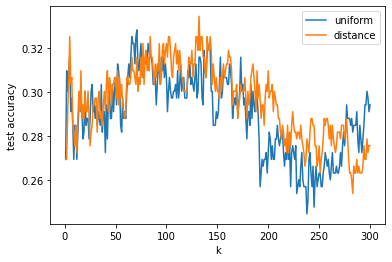
\includegraphics[width=0.8\linewidth]{kNN_trend.png}
\caption{The number of neighbours vs. the test matrix accuracy both for uniformly weighted kNN and distance-based weighted kNN}
\label{kNN_trend}
\end{figure}

From Figure \ref{kNN_trend}, we observe that distance-based weighted kNN outperforms the uniformly weighted kNN.  Compared to uniformly weight method, which causes miss-classification after adding too many neighbours, the distance-based weighted kNN can decrease the overfitting by adding more neighbours to the checking set, which results in higher testing accuracy. 

We use the kNN implemented in scikit-learn package. We present the best model we can fit using kNN classification method as follows:

\noindent  for $lag = 3$:
\smallskip\\
Variables: \textit{GSPC\_log\_ret}, \textit{BTC\_log\_ret}, \textit{NVDA\_log\_ret}, \textit{Gold\_log\_ret}, \textit{US\_inflation\_rate}, \textit{3\_month\_LIBOR}. 6 variables, thus $6\times lag$ features.\\
Parameters: \textit{n\_neighbours=64},\textit{weights='distance'}
\smallskip\\
Testing:

\begin{center}
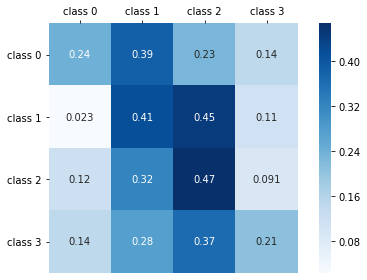
\includegraphics[scale=0.35]{kNN_test.png}
%\label{kNN_test}
\end{center}

From the confusion matrix, we observe that the heatmap of our confusion matrix is more diagonalized, which means that the median labelling method helps to identify more data points in the budget. But the overall confusion matrix accuracy for kNN, which is 33.34\%, is lower than SVC model.

\section{Predicting Bitcoin Log Return via Random Forest (RF)}

Then we consider Random Forest as another option to reduce over-fitting in this multi-class classification problem. Random forests are a meta estimator that apply decision trees classifiers on subset and use averaging to generate the final prediction. The training algorithm for random forests involves the technique of bootstrap aggregating, or bagging.
For the bagging technique, given a training set $X = x_1,x_2,...,x_n$ with responses $Y = y_1,y_2,...,y_n$ bagging repeatedly selects a random sample with replacement of training set and fits trees to these samples \cite{lin2006random}.

\hspace{2mm} For $b=1,2,...,B$

\hspace{4mm}1. Sample $n$ training samples with replacement from $X,Y$, generate $X_b, Y_b$.

\hspace{4mm}2. Train a decision tree $f_b$ on $X_b, Y_b$.

\hspace{2mm} Predict the test data point $x'$ by averaging the predictions from all the individual regression trees on $x'$:

\[
y'_{pred}=\frac{1}{B} \dot \sum_{b=1}^B f_b(x')
\]

We use the Random Forest implemented in scikit-learn package. We present the best model we can fit using random forest classification method as following:

\noindent  for $lag = 3$:
\smallskip\\
Variables: \textit{GSPC\_log\_ret}, \textit{BTC\_log\_ret}, \textit{NVDA\_log\_ret}, \textit{Gold\_log\_ret}, \textit{US\_inflation\_rate}, \textit{3\_month\_LIBOR}. 6 variables, thus $6\times lag$ features.
Parameters: \textit{max\_depth=33}
\smallskip\\
Testing:

\begin{center}
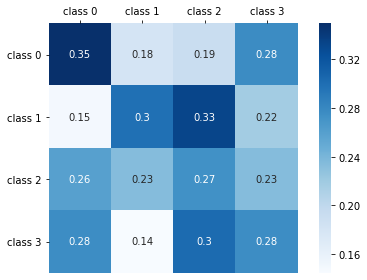
\includegraphics[scale=0.35]{rf_test.png}
%\label{rf_test}
\end{center}

From the confusion matrix, we observe that our confusion matrix for our Random Forest model is more scattered than the kNN output. The best accuracy taking the last 20\% data set as the test data set is 32.20\% which indicates Random Forest does not perform well on this classification problem compared to SVC and kNN.

\section{Discussion and Conclusion}
\subsection*{Predicting Bitcoin Pricing is Hard}
"The crypto ecosystem, like any other financial market, depends on too many variables to permit accurate predictions. From political decisions and new crypto-products being launched to psychological factors – anything can impact the price."
\\[3pt]
--- How reliable is a Bitcoin price prediction? Yahoo Finance, Christina Comben and Coin Rivet. October 3, 2019
\\[3pt]

In real life, the financial market is dependent on too many variables to ensure reliable predictions. For bitcoin, from political decisions and new crypto-products being launched to psychological factors – anything can impact the price of bitcoin. For example, Chinese regulatory authorities termed initial coin offerings (ICO), a cryptocurrency-based fundraising process, illegal in China September 2017. That ban triggered an instant 6\% decline in bitcoin prices. On the other hand, value of bitcoin raised by 26.5\% since President Trump announced he would raise tariffs on Chinese imports by May 17, 2019. There is no way we can capture such impact with our model. 

In conclusion, our models, are relatively simple and naive, mostly due to the lack of accessible data and partially due to the model simplicity. We do not feel confident implementing any of these models in all scenarios. However, if we were to implement any of these models in production, we would consider the probabilistic approach utilizing a quantile regression to make short term speculation on data points that fall within our confidence interval.

\subsection*{Weapons of Math Destruction (WMD) and Fairness}
If our model predicted bitcoin returns with some probability reliably above 50 percent net of trading costs, our model would be considered by some observers as a weapon of math destruction.  We consider the three attributes of WMD's below.

The outcome of our model is testable. This can be seen as our model will predict either a positive or negative return, which can be compared with the true value at the end of each trading day.

Predictions by our model would influence bitcoin returns. To show this, we suppose that all humans are rational and that our model predicts a positive return. It follows that investors would increase demand to purchase bitcoin and sellers would decrease the supply of selling bitcoin as each would want to hold on to the bitcoin for the predicted positive return. By the law of supply and demand, the price of bitcoin would then rise completing the self fulfilling prophecy. Conversely, if our model predicted a negative return for bitcoin, investors would decrease their demand to purchase bitcoin while current holders would be more willing to sell their current bitcoin, which by the law of supply and demand would cause the price of bitcoin to decline. Thus again completing the self fulfilling prophecy.
Our model would also have the potential for harmful impacts on users as our model will not predict with perfect certainty that returns will be positive or negative. Therefore it follows that investors could face short term losses in the case our model outputs a false positive prediction.

We do not believe fairness is an important criterion to be considered when choosing a model for application.

\subsection*{Summary}
In this report, we have first introduce the problem of the prediction of bitcoin pricing. Then we present the explanatory variables that have the potential in predicting the bitcoin pricing.

We do an exploratory data analysis with the data set we built, together with preliminary linear regression and quantile regression with lag features. Using the quantile regression, we can predict the bitcoin price on the 1-day-prior basis, with confidence in whether the predicted value is higher/lower than the true value. 

Then we come to the analysis of the stationarity of the bitcoin pricing and the log returns. We find out that the pricing is not stationary, but the log return is. This helps us to re-formalize the problem into a multi-class classification problem. 

We employ support vector classifier with RBF and polynomial kernels, the kNN method, and the random forest method to approach the multi-class classification problem. Different labeling strategies are used. Though the classification models cannot classify all the test data well, they can classify some of the classes with a decent confidence.

% Bibliography

\bibliography{bibliography}

\end{document}